% =====================================================================
%  WheelsEye: Label-Free Per-Driver Calibration for Subject-Independent
%  Multimodal Drowsiness Detection
%  -------------------------------------------------------------------
%  Single-file, Overleaf-ready IEEE journal (T-ITS) manuscript.
%  * Compile with pdfLaTeX (2 passes). No external figure files: every
%    figure (architecture diagram, protocol ladder, leakage-control
%    bars, regime slope chart, dual-transform enrollment curve,
%    per-driver split violins with paired lines, per-class recall,
%    RLDD bars, inflation bars) is drawn with TikZ/pgfplots from the
%    numbers reported in the tables. Violin densities were computed
%    offline (Gaussian kernel, Silverman bandwidth) and embedded.
%  * TODO (authors): fill in real names, e-mails, and the manuscript
%    received/funding notes in \author{} and \thanks{}.
%  * All placeholders resolved; values from revision_results_v2exact/
%    that must come from your pipeline. Run wheelseye_revision_controls.py
%    on the V2 feature table; it prints paste-ready table rows.
%  * Per-driver values are the exact per-subject accuracies from the
%    authors' v3 results (z-score 4-min enrollment; Table XI there).
% =====================================================================
\documentclass[journal]{IEEEtran}

\usepackage{cite}
\usepackage{url}
\usepackage{amsmath,amssymb,amsfonts}
\usepackage{graphicx}
\usepackage{xcolor}
\usepackage{booktabs}
\usepackage{multirow}
\usepackage{threeparttable}
\usepackage{balance}
\usepackage{tikz}
\usetikzlibrary{arrows.meta,positioning,calc,fit,backgrounds,shapes.misc}
\usepackage{pgfplots}
\pgfplotsset{compat=1.18}

% ---------- palette (colour-blind tolerant, print safe) ----------
\definecolor{weBlue}{RGB}{31,119,180}
\definecolor{weOrange}{RGB}{255,127,14}
\definecolor{weGreen}{RGB}{44,160,44}
\definecolor{weRed}{RGB}{214,39,40}
\definecolor{weOlive}{RGB}{150,150,30}
\definecolor{wePurple}{RGB}{148,103,189}
\definecolor{weBrown}{RGB}{140,86,75}
\definecolor{weGray}{RGB}{110,110,110}

% ---------- shared chart style ----------
\pgfplotsset{
  wechart/.style={
    tick label style={font=\scriptsize},
    label style={font=\scriptsize},
    title style={font=\scriptsize\bfseries},
    legend style={font=\tiny,draw=weGray!40,fill=white,fill opacity=0.9,text opacity=1},
    ymajorgrids,
    grid style={weGray!22},
    axis line style={weGray!70},
    tick style={weGray!70},
    every node near coord/.append style={font=\tiny},
  }
}

\newcommand{\pp}{\,pp}
% placeholder macros retired -- all values resolved
\newcommand{\sysname}{WheelsEye}
\newcommand{\rone}{R1}
\newcommand{\rtwo}{R2}
\newcommand{\rthree}{R3}

\begin{document}

\title{\sysname: Label-Free Per-Driver Calibration for\\
Subject-Independent Multimodal Drowsiness Detection}

\author{Author~One, Author~Two, Author~Three, Author~Four, and~Faculty~Mentor%
\thanks{Manuscript received September 4, 2026. (TODO: funding, corresponding
author, and revision notes.)}%
\thanks{The authors are with the Computer Science and Engineering Department,
Thapar Institute of Engineering and Technology, Patiala 147004, India
(e-mail: author.emails@thapar.edu).}}

\markboth{IEEE Transactions on Intelligent Transportation Systems}%
{One \MakeLowercase{\textit{et al.}}: \sysname: Label-Free Per-Driver Calibration for Subject-Independent Multimodal Drowsiness Detection}

\maketitle

\begin{abstract}
Multimodal driver drowsiness detectors report high accuracy under
subject-mixed cross-validation. We show that this protocol measures
memorization: with labels randomly permuted within four-minute blocks a model
still scores 98.7\%, and a single 10-s window identifies the driver. \sysname{} treats the
evaluation protocol as an experimental factor and pairs it with personalization
a deployed device can perform. Six
architectures are scored on byte-identical, audited splits of the UL-DD
benchmark under window-mixed, temporally blocked and leave-one-subject-out
regimes. Each sensor feature is then expressed relative to the mean of the
driver's first eight minutes of alert driving, obtained once at enrollment
without labels. This offset removal raises unseen-driver accuracy
by 28.4 percentage points ($p<0.0001$, 16 of 16 drivers) and recovers all
three severity classes; z-scoring trails by ten points on this fixed-rig
dataset, and transductive alternatives that use more of the driver's data fall
below the short enrollment. A $2^{6}$ modality lattice attributes the
calibrated signal to facial action units and autonomic channels, plus a
drive-relative context term that controls show to be temporal; cardiac and
grip channels add nothing. The effect
replicates on MePhy and on RLDD, where 59 subjects filmed themselves on their
own devices and gain 15.6\pp{} with enrollment windows excluded from scoring;
RLDD has no session-time structure, so the mechanism holds where a clock cannot
predict the label. Under identical calibration a 2-MB
gradient-boosted model surpasses every fusion architecture at 0.86\,ms per
window. Protocol, enrollment and sensor choice, not model capacity, determine
what a deployed detector can achieve.
\end{abstract}

\begin{IEEEkeywords}
Driver drowsiness detection, multimodal fusion, leave-one-subject-out,
evaluation leakage, per-driver calibration, personalization, LightGBM,
edge deployment, UL-DD.
\end{IEEEkeywords}

% =====================================================================
\section{Introduction}
% =====================================================================
\IEEEPARstart{D}{river} fatigue contributes to 10 to 25\% of road crashes in
the European Union. Since July~2024, every newly registered car, bus and truck
there must carry a driver drowsiness and attention warning (DDAW) system, and
its type approval is validated on human participants against the Karolinska
Sleepiness Scale (KSS)~\cite{eu2021ddaw,akerstedt1990kss}. Drowsiness
detection has therefore become a shipped safety function. The question a
manufacturer must answer is not whether a model recognizes a driver it has
already seen, but whether it detects drowsiness in a driver it has never met.

Most of the research literature has answered a different question.
Multimodal datasets that pair in-cabin video with wearable physiology and
behavioural signals~\cite{bodaghi2026uldd,ortega2020dmd,massoz2016drozy} have
enabled elaborate fusion architectures, including graph neural networks with
transformer encoders and learned gating~\cite{zendehbad2025fatiguenet},
product-of-experts models of inter- and intra-modality
dependencies~\cite{madaan2024i2m2} and attention-based self-supervised
fusion~\cite{mou2023isotropic}. Reported accuracies range from 85\% to 99\%.
On UL-DD~\cite{bodaghi2026uldd}, the richest such benchmark, published
baselines reach 83.75\% (SVM) and 88.03\% (I2M2). All of these figures come
from stratified cross-validation with every subject present in every training
fold. Physiological windows overlap, and labels stay constant over four-minute
KSS intervals. Such a split therefore places a temporal neighbour of each test
window, with nearly identical features and the same label, in the training
set. The evaluation then certifies that the driver and the moment can be
recognized. It says almost nothing about an unseen driver.

Similar failure modes are known in neighbouring fields. Examples are the
pairwise-similarity bias in activity recognition~\cite{hammerla2015stick},
the general leakage taxonomy of Kapoor and Narayanan~\cite{kapoor2023leakage}
and the persistent gap between within-subject and cross-subject accuracy in
EEG vigilance estimation~\cite{cui2022compact,shen2021subject}. For
multimodal drowsiness detection, however, the size of the gap, the mechanisms
behind it and the performance that remains once it is closed have not been
measured on one benchmark with everything else held fixed. Three obstacles
make this measurement hard. The first is inter-driver offset. Resting heart
rate, electrodermal level and skin temperature differ more between people than
between the alert and drowsy states of one person, so a model trained on
absolute values reads some alert drivers as drowsy from their first minute.
The second is small cohorts. With 16 evaluable drivers, standard errors span
several points and apparently clear differences are often not significant.
The third is hidden transduction. Personalization schemes that normalize a
driver with statistics of the very session being scored gain accuracy through
session identity, and the gain stays invisible unless the amount of adaptation
data is varied.

\sysname{} (Fig.~\ref{fig:arch}) addresses these obstacles. It treats the
evaluation protocol as an experimental factor and pairs it with
personalization that a shipped device can perform. Six architectures consume
one 135-dimensional feature table under three regimes that are persisted once
as fold files, namely window-mixed (\rone), temporally blocked known-driver
(\rtwo) and leave-one-subject-out (\rthree, LOSO). Machine-checked invariants
ensure that no held-out driver contributes to any statistic. A label-free
calibration expresses each sensor feature relative to statistics of the
driver's first $k$ minutes of alert driving, with mean subtraction as the
primary transform and z-scoring as a variant. Label-free here means that no
drowsiness label is ever read. The method does assume that the enrollment
period is alert, which is a protocol assumption rather than a label, and we
test what happens when that assumption is violated
(Sec.~\ref{sec:controls2}). The enrollment mirrors a one-time procedure on a
shipped device. We sweep $k$ from one minute to the whole
session to separate genuine baseline estimation from transductive
self-standardization, and we exclude the enrollment windows from scoring
wherever they form a large share of the test set. The contributions are as
follows.
\begin{itemize}
\item \textbf{Deployment-tiered evaluation with audited splits and direct
controls.} The three regimes are consumed byte-identically by every model.
Three pipeline leakage mechanisms are quantified, namely checkpoint selection
on the test subject, full-table normalization and shared training sets across
folds. Two controls, block-permuted labels and single-window driver
identification, show that the subject-mixed protocol of prior work rewards
memorization and driver identity rather than drowsiness.
\item \textbf{Label-free per-driver offset removal, audited for transduction
and for scoring shortcuts.} Subtracting a per-feature mean computed once from
a few minutes of unlabelled alert driving is the largest single effect we
measure. It recovers all three severity classes, including the transitional
one, and approaches a supervised-enrollment bound. Sweeping the enrollment
length for both transforms shows that session-long z-score baselines help
only once they contain the scored windows, whereas under mean subtraction a
brief and fresh enrollment is best. Transductive alternatives with strictly
more driver data fall below the short enrollment. We also measure the accuracy
gained by scoring the enrollment windows themselves and show that it grows
with their share of the test set.
\item \textbf{Replication on three datasets and a rule for the transform.}
The effect holds on MePhy (physiological sensors, four classes) and on RLDD
(59 subjects, own-device webcam video, binary task). The two datasets disagree
on whether to divide by the per-subject standard deviation, and the
disagreement tracks the recording setup. Fixed instruments call for mean
subtraction. Own devices call for full standardization.
\item \textbf{Subject-independent modality attribution and matched-condition
architecture findings.} A $2^{6}$ sensor-group lattice under identical
calibration attributes the signal to facial action units and autonomic
channels, with a further contribution from drive-relative context that a
time-on-task control shows to be temporal in nature; cardiac and grip features
contribute nothing. This reverses both the base benchmark's fusion narrative
and our own earlier wristband-first recommendation. With identical features,
folds and calibration, a compact gradient-boosted model exceeds
graph-transformer, product-of-experts, attention and ensemble baselines, and a
leakage-controlled ablation traces the transferable part of the fusion
architecture to temporal attention alone.
\end{itemize}
Taken together, the results say that the binding constraints for in-cab
drowsiness detection are the evaluation protocol, a few minutes of label-free
enrollment and the choice of sensors, not model capacity.

% =====================================================================
\section{Related Work}
% =====================================================================
\subsection{Multimodal Driver Drowsiness Detection}
Public benchmarks have moved from single-camera video to multi-sensor
recordings. NTHU-DDD contains acted drowsiness~\cite{weng2017nthu}. UTA-RLDD
has 60 subjects who recorded about 30~h of real-life video on their own
devices at three vigilance levels~\cite{ghoddoosian2019uta}. DROZY pairs video
with polysomnographic signals and KSS~\cite{massoz2016drozy}. SEED-VIG couples
EEG with forehead EOG for continuous vigilance
estimation~\cite{zheng2017vigilance}. DMD provides 41~h of RGB, depth and
infrared video of 37 drivers~\cite{ortega2020dmd}. UL-DD~\cite{bodaghi2026uldd}
adds a wristband, a pulse oximeter, steering-grip pressure and simulator
telemetry across two 40-minute sessions per driver. Recent
surveys~\cite{fu2024survey,albadawi2022review,saleem2023review} document the
modelling trend that came with these datasets, from hand-crafted ocular
measures such as PERCLOS to deep video models, and from single physiological
channels, of which heart-rate variability is the best
studied~\cite{lu2022hrv,jiao2024hrveda}, to learned multimodal fusion.
Examples of fusion are attention-based fusion trained with
self-supervision~\cite{mou2023isotropic}, FatigueNet's dynamic sensor graph
with a transformer encoder and meta-learned gates~\cite{zendehbad2025fatiguenet}
and the product-of-experts model I2M2~\cite{madaan2024i2m2}. Almost all of
this work reports subject-mixed cross-validation. Whether the reported gains,
or the architectures that produce them, survive a held-out driver has not been
established on a common footing.

\subsection{Subject-Independent Evaluation and Leakage}
Hammerla and Pl\"otz showed that random cross-validation over overlapping
sensor frames is biased upward. Temporally adjacent frames are near-identical,
so user-dependent accuracy under such splits is not even an upper bound on
real performance~\cite{hammerla2015stick}. Kapoor and Narayanan catalogued
eight leakage types across 294 papers in 17 fields, among them preprocessing
on the full dataset, temporal leakage and non-independence between train and
test samples~\cite{kapoor2023leakage}. In clinical machine learning on
wearable data, Saeb et al.\ showed that record-wise cross-validation grossly
overstates the accuracy of subject-wise use~\cite{saeb2017usecase}, and the
ensuing exchange clarified which question each strategy
answers~\cite{little2017crossval}. In EEG-based vigilance estimation the
consequence is familiar. Calibration-free cross-subject accuracy is far below
within-subject figures~\cite{cui2022compact}, which has motivated
subject-independent feature alignment~\cite{shen2021subject}, adversarial
domain generalization~\cite{ma2019depersonalized} and inter-subject
transfer~\cite{liu2020intersubject}. For multimodal video-plus-wearable
drowsiness detection, the leakage has been neither quantified nor decomposed.
Window-level, subject-level and pipeline-level mechanisms (normalization
statistics, checkpoint selection, fold construction) act at the same time and
are rarely audited. \sysname{} separates them on one benchmark with
byte-identical splits and machine-checked invariants.

\subsection{Personalization and Efficient Deployment}
Between-person variation of physiological baselines is the main obstacle to
cross-subject transfer. The usual remedies adapt the model to the target
person through inter-subject transfer learning~\cite{liu2020intersubject},
adversarial domain generalization~\cite{ma2019depersonalized} or, in a recent
multimodal fatigue system, online personalized fine-tuning with sensor-quality
gating~\cite{aravinth2025dynamic}. A label-free alternative is test-time
distribution alignment such as CORAL~\cite{sun2016coral}, which matches the
second-order statistics of the target to the source. These approaches need
labelled target data, or unlabelled target data plus parameter updates on the
device, and their evaluations rarely say how much of the scored session was
used for adaptation. Per-subject normalization of features is itself an old
idea in affective computing. What has been missing is an audit of how much
target data it uses, whether that data is scored, and when the scale should be
removed as well as the offset. We take the simplest design point, a fixed
model and a feature-space transform computed once from minutes of unlabelled
alert data, and we treat the enrollment length and the scoring convention as
experimental variables. On the modelling side, gradient-boosted decision trees
(GBDTs) remain state of the art on medium-sized tabular data and tolerate
uninformative features well~\cite{grinsztajn2022tree,shwartz2022tabular}.
LightGBM's histogram-based, leaf-wise growth gives particularly compact
models~\cite{ke2017lightgbm}. A DDAW function must run for the entire drive
on in-vehicle hardware shared with camera pipelines~\cite{eu2021ddaw}, yet
prior studies seldom report footprint next to subject-independent accuracy. We
report model size and latency for the deployed configuration
(Sec.~\ref{sec:efficiency}).

% =====================================================================
\section{The \sysname{} Framework}
% =====================================================================
Fig.~\ref{fig:arch} summarizes \sysname. The top half is a deployment
pipeline made of sensing, windowing, feature extraction, label-free per-driver
calibration and a lightweight classifier. The bottom half is a
deployment-tiered evaluation design that scores the same model and features
under three regimes on audited, byte-identical splits.

\begin{figure*}[!t]
\centering
\resizebox{\textwidth}{!}{%
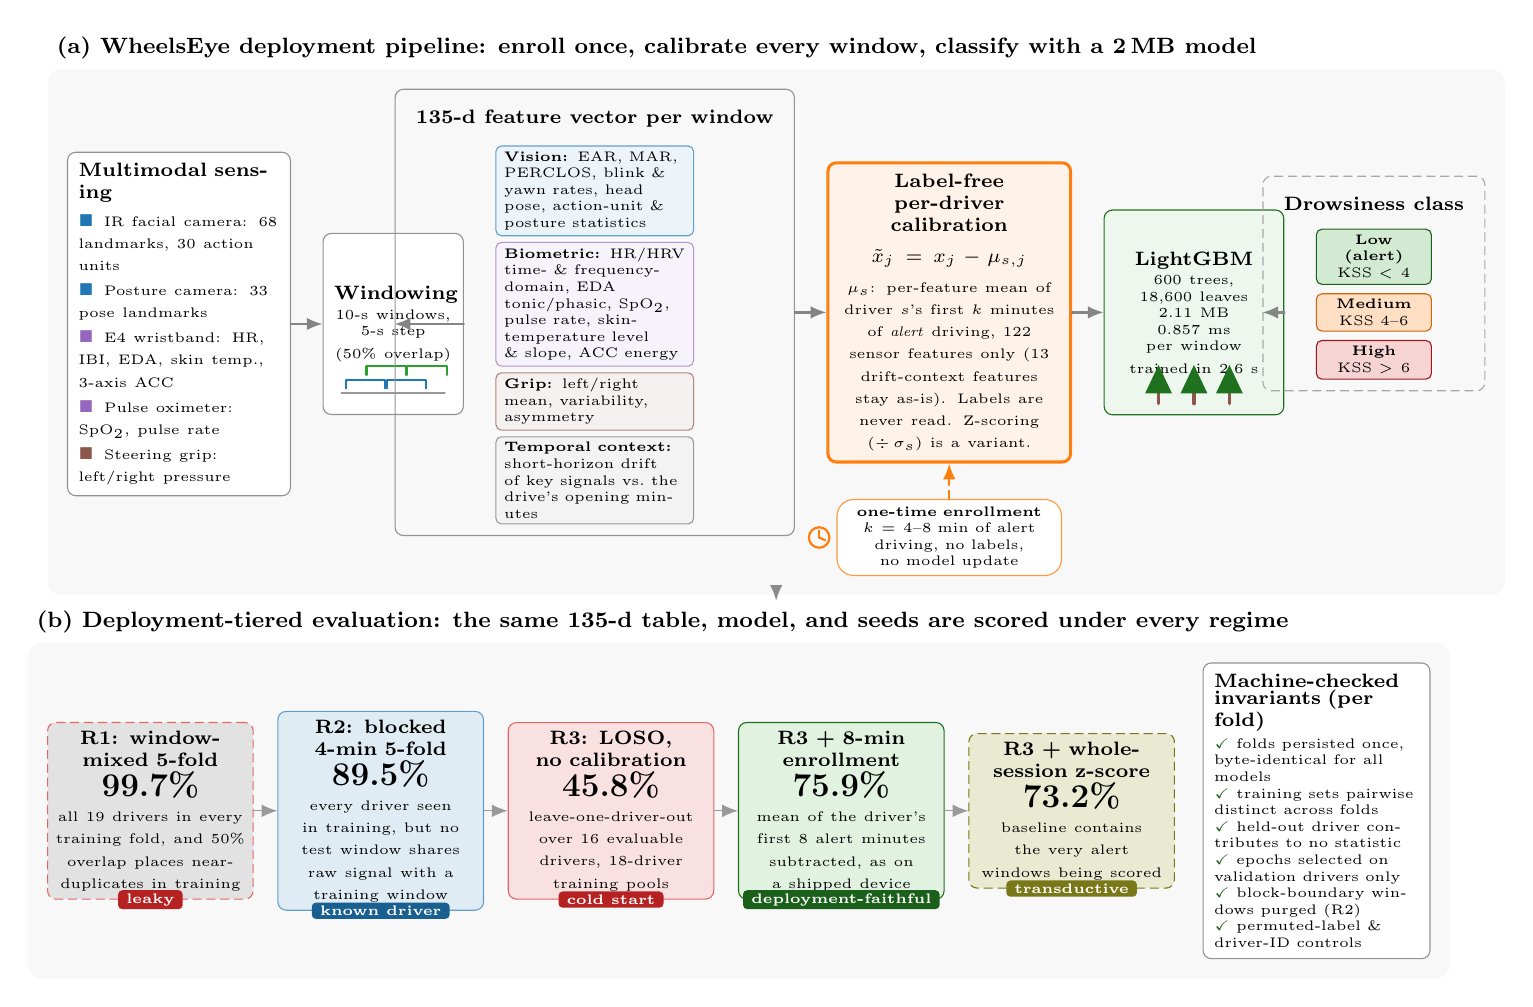
\begin{tikzpicture}[
  font=\scriptsize,
  >={Latex[length=2mm,width=1.6mm]},
  line cap=round, line join=round,
  stage/.style={draw=weGray!75, fill=white, rounded corners=3pt, align=center, inner sep=4pt},
  chip/.style={draw, rounded corners=2pt, inner xsep=3pt, inner ysep=2pt, align=left, font=\tiny, text width=2.3cm},
  ochip/.style={draw, rounded corners=2pt, inner xsep=3pt, inner ysep=2pt, align=center, font=\tiny, text width=1.25cm},
  tag/.style={rounded corners=1.5pt, inner xsep=3pt, inner ysep=1.2pt, font=\tiny\bfseries, text=white},
  flow/.style={->, thick, weGray!85},
  card/.style={draw, rounded corners=3pt, align=center, inner sep=3pt, text width=2.4cm, minimum height=1.8cm},
]
% ================= (a) deployment pipeline =================
\node[stage, align=left, text width=2.55cm] (S) {%
  \textbf{Multimodal sensing}\\[2pt]
  {\tiny\textcolor{weBlue}{$\blacksquare$}\, IR facial camera: 68 landmarks, 30 action units}\\[1pt]
  {\tiny\textcolor{weBlue}{$\blacksquare$}\, Posture camera: 33 pose landmarks}\\[1pt]
  {\tiny\textcolor{wePurple}{$\blacksquare$}\, E4 wristband: HR, IBI, EDA, skin temp., 3-axis ACC}\\[1pt]
  {\tiny\textcolor{wePurple}{$\blacksquare$}\, Pulse oximeter: SpO$_2$, pulse rate}\\[1pt]
  {\tiny\textcolor{weBrown}{$\blacksquare$}\, Steering grip: left/right pressure}};

\node[stage, right=0.4cm of S, text width=1.5cm, minimum height=2.3cm] (W) {%
  \textbf{Windowing}\\[1pt]{\tiny 10-s windows,\\5-s step\\(50\% overlap)}\\[18pt]};
\begin{scope}[shift={($(W.south)+(0,0.30)$)}]
  \draw[weGray!70] (-0.66,-0.02) -- (0.66,-0.02);
  \foreach \x/\c/\y in {-0.60/weBlue/0,-0.34/weGreen/0.17,-0.08/weBlue/0,0.18/weGreen/0.17}{%
    \draw[\c, thick] (\x,\y+0.04) -- (\x,\y+0.15) -- (\x+0.50,\y+0.15) -- (\x+0.50,\y+0.04);}
\end{scope}

\node[chip, draw=wePurple!70, fill=wePurple!8, right=0.4cm of W, yshift=0.25cm] (cB)
  {\textbf{Biometric:} HR/HRV time- \& frequency-domain, EDA tonic/phasic, SpO$_2$, pulse rate, skin-temperature level \& slope, ACC energy};
\node[chip, draw=weBlue!70, fill=weBlue!8, above=2pt of cB] (cV)
  {\textbf{Vision:} EAR, MAR, PERCLOS, blink \& yawn rates, head pose, action-unit \& posture statistics};
\node[chip, draw=weBrown!70, fill=weBrown!8, below=2pt of cB] (cG)
  {\textbf{Grip:} left/right mean, variability, asymmetry};
\node[chip, draw=weGray!70, fill=weGray!8, below=2pt of cG] (cC)
  {\textbf{Temporal context:} short-horizon drift of key signals vs.\ the drive's opening minutes};
\node[font=\scriptsize\bfseries, above=3pt of cV] (tF) {135-d feature vector per window};
\node[stage, fill=none, fit=(tF)(cV)(cB)(cG)(cC)] (F) {};

\node[stage, draw=weOrange, line width=1.1pt, fill=weOrange!9, right=0.4cm of F, text width=2.8cm, minimum height=2.6cm] (C) {%
  \textbf{Label-free}\\\textbf{per-driver calibration}\\[3pt]
  $\displaystyle \tilde{x}_{j}=x_{j}-\mu_{s,j}$\\[3pt]
  {\tiny $\mu_{s}$: per-feature mean of driver $s$'s first $k$ minutes of \emph{alert} driving, 122 sensor features only (13 drift-context features stay as-is).
  Labels are never read. Z-scoring ($\div\,\sigma_{s}$) is a variant.}};

\node[draw=weOrange!80, fill=white, rounded corners=6pt, inner xsep=5pt, inner ysep=2.5pt, font=\tiny,
      below=0.45cm of C, text width=2.5cm, align=center] (E)
  {\textbf{one-time enrollment}\\$k=4$--$8$ min of alert driving, no labels, no model update};
\draw[->, weOrange, thick, densely dashed] (E.north) -- (C.south);
\begin{scope}[shift={($(E.west)+(-0.22,0)$)}]
  \draw[weOrange, thick] (0,0) circle (0.13);
  \draw[weOrange, thick] (0,0) -- (0,0.09);
  \draw[weOrange, thick] (0,0) -- (0.075,-0.035);
\end{scope}

\node[stage, draw=weGreen!70!black, fill=weGreen!8, right=0.4cm of C, text width=2.0cm, minimum height=2.6cm] (M) {%
  \textbf{LightGBM}\\[1pt]{\tiny 600 trees, 18{,}600 leaves\\2.11 MB\\0.857 ms per window\\trained in 2.6 s}\\[20pt]};
\begin{scope}[shift={($(M.south)+(0,0.28)$)}]
  \foreach \x in {-0.45,0,0.45}{%
    \draw[weBrown, line width=1.3pt] (\x,-0.13) -- (\x,0.02);
    \fill[weGreen!70!black] (\x-0.17,0) -- (\x,0.36) -- (\x+0.17,0) -- cycle;}
\end{scope}

\node[ochip, fill=weOrange!25, draw=weOrange!80!black, right=0.4cm of M] (oM) {\textbf{Medium}\\KSS 4--6};
\node[ochip, fill=weGreen!22, draw=weGreen!60!black, above=3pt of oM] (oL) {\textbf{Low (alert)}\\KSS $<4$};
\node[ochip, fill=weRed!20, draw=weRed!70!black, below=3pt of oM] (oH) {\textbf{High}\\KSS $>6$};
\node[font=\scriptsize\bfseries, above=3pt of oL] (tO) {Drowsiness class};
\node[stage, fill=none, densely dashed, draw=weGray!60, fit=(tO)(oL)(oM)(oH)] (O) {};

\draw[flow] (S.east) -- (S.east -| W.west);
\draw[flow] (W.east) -- (W.east -| F.west);
\draw[flow] (F.east) -- (F.east -| C.west);
\draw[flow] (C.east) -- (C.east -| M.west);
\draw[flow] (M.east) -- (M.east -| O.west);

\begin{scope}[on background layer]
  \node[fill=weGray!5, rounded corners=5pt, inner sep=7pt, fit=(S)(W)(F)(C)(M)(O)(E)] (TOP) {};
\end{scope}
\node[font=\footnotesize\bfseries, anchor=south west] at (TOP.north west)
  {(a) \sysname{} deployment pipeline: enroll once, calibrate every window, classify with a 2\,MB model};

% ================= (b) deployment-tiered evaluation =================
\node[card, draw=weRed!70, densely dashed, fill=weGray!20, below=1.6cm of TOP.south west, anchor=north west] (r1)
  {\textbf{\rone: window-mixed 5-fold}\\[1pt]{\large\bfseries 99.7\%}\\[1pt]{\tiny all 19 drivers in every training fold, and 50\% overlap places near-duplicates in training}};
\node[card, draw=weBlue!70, fill=weBlue!14, right=0.3cm of r1] (r2)
  {\textbf{\rtwo: blocked 4-min 5-fold}\\[1pt]{\large\bfseries 89.5\%}\\[1pt]{\tiny every driver seen in training, but no test window shares raw signal with a training window}};
\node[card, draw=weRed!70, fill=weRed!14, right=0.3cm of r2] (r3)
  {\textbf{\rthree: LOSO, no calibration}\\[1pt]{\large\bfseries 45.8\%}\\[1pt]{\tiny leave-one-driver-out over 16 evaluable drivers, 18-driver training pools}};
\node[card, draw=weGreen!70!black, fill=weGreen!14, right=0.3cm of r3] (r4)
  {\textbf{\rthree{} + 8-min enrollment}\\[1pt]{\large\bfseries 75.9\%}\\[1pt]{\tiny mean of the driver's first 8 alert minutes subtracted, as on a shipped device}};
\node[card, draw=weOlive!80!black, densely dashed, fill=weOlive!20, right=0.3cm of r4] (r5)
  {\textbf{\rthree{} + whole-session z-score}\\[1pt]{\large\bfseries 73.2\%}\\[1pt]{\tiny baseline contains the very alert windows being scored}};
\node[tag, fill=weRed!85!black] at (r1.south) {leaky};
\node[tag, fill=weBlue!80!black] at (r2.south) {known driver};
\node[tag, fill=weRed!85!black] at (r3.south) {cold start};
\node[tag, fill=weGreen!60!black] at (r4.south) {deployment-faithful};
\node[tag, fill=weOlive!80!black] at (r5.south) {transductive};
\foreach \a/\b in {r1/r2,r2/r3,r3/r4,r4/r5}{\draw[->, weGray!70] (\a) -- (\b);}

\node[stage, align=left, right=0.35cm of r5, text width=2.6cm, minimum height=1.8cm, font=\tiny] (A) {%
  {\scriptsize\textbf{Machine-checked}}\\{\scriptsize\textbf{invariants (per fold)}}\\[2pt]
  \textcolor{weGreen!60!black}{$\checkmark$} folds persisted once, byte-identical for all models\\
  \textcolor{weGreen!60!black}{$\checkmark$} training sets pairwise distinct across folds\\
  \textcolor{weGreen!60!black}{$\checkmark$} held-out driver contributes to no statistic\\
  \textcolor{weGreen!60!black}{$\checkmark$} epochs selected on validation drivers only\\
  \textcolor{weGreen!60!black}{$\checkmark$} block-boundary windows purged (\rtwo)\\
  \textcolor{weGreen!60!black}{$\checkmark$} permuted-label \& driver-ID controls};

\begin{scope}[on background layer]
  \node[fill=weGray!5, rounded corners=5pt, inner sep=7pt, fit=(r1)(r5)(A)] (BOT) {};
\end{scope}
\node[font=\footnotesize\bfseries, anchor=south west] (lbB) at (BOT.north west)
  {(b) Deployment-tiered evaluation: the same 135-d table, model, and seeds are scored under every regime};
\draw[->, weGray!80, thick, densely dashed] (TOP.south) -- (TOP.south |- lbB.north);
\end{tikzpicture}}
\caption{The \sysname{} system and evaluation design. \textbf{(a)}~Five sensor
streams are cut into 10-s windows with a 5-s step and summarized as a 135-d
feature vector in four groups. Each of the 122 sensor features is expressed
relative to the mean of the driver's own first $k$ minutes of alert driving.
This mean is computed once at enrollment, without labels or model updates. A
600-tree LightGBM then assigns one of three KSS bins. Z-scoring is evaluated as
a variant. \textbf{(b)}~The same model and feature table are scored under
three regimes on byte-identical, audited folds, backed by permuted-label and
driver-identification controls. One model spans 54 percentage points across
regimes, so every number in this paper belongs to a (model, protocol) pair.
The colours in (b) are reused in Fig.~\ref{fig:ladder}.}
\label{fig:arch}
\end{figure*}

\subsection{Datasets, Labels and Features}
\label{sec:data}
UL-DD~\cite{bodaghi2026uldd} is the primary benchmark. It has 19 subjects (15
male, 4 female) who drove a fixed-base simulator (American Truck Simulator)
for two 40-minute sessions, one entered alert and one entered drowsy (KSS
$\ge 6$ was required to start). The streams are an infrared facial camera (68
facial landmarks, 30 action units), a posture camera (33 pose landmarks), an
Empatica~E4 wristband (heart rate, inter-beat intervals, electrodermal
activity, skin temperature, acceleration), a pulse oximeter and two
steering-grip pressure sensors. KSS self-reports every four minutes are binned
exactly as in~\cite{bodaghi2026uldd}, with Low below 4, Medium from 4 to 6
and High above 6. Formally, each window $i$ is a tuple
$(\mathbf{x}_i,y_i,s_i,t_i)$ with features $\mathbf{x}_i\in\mathbb{R}^{135}$,
label $y_i\in\{\text{Low},\text{Medium},\text{High}\}$, driver $s_i$ and
session time $t_i$. The deployment question is the accuracy of
$\hat y(\mathbf{x})$ on windows whose driver never appears in training. Three
subjects (C, F, L) completed only the alert session. They have no High-class
support and are never held out, but their windows stay in every training
pool. This gives 16 evaluable subjects and 18-subject training pools under
LOSO. Simulator telemetry (speed, heading) is excluded because no deployable
in-cab sensor produces it.

All modalities are cut into 10-s windows with a 5-s step. The window grid of
each session is set by its shortest fully covered modality. Each window yields
135 features in four groups (Fig.~\ref{fig:arch}a). The \emph{vision} group
holds ocular and mouth geometry, PERCLOS, blink and yawn rates, head pose and
action-unit and posture statistics. The \emph{biometric} group holds
heart-rate and HRV time- and frequency-domain measures, tonic and phasic
electrodermal components, SpO$_2$ and pulse-rate statistics, skin-temperature
level and slope and accelerometer energy. The \emph{grip} group holds
left/right level, variability and asymmetry. The \emph{temporal context}
group holds the short-horizon drift of key signals relative to the opening
minutes of the current drive. Features are computed once and persisted, and
every model consumes the same table of 16{,}671 windows. We call this the V2
feature set. A 37-feature first-generation set (V1), on which the leakage
measurements of Sec.~\ref{sec:leakage} were made, is used only where stated.

Two further datasets test the calibration mechanism. MePhy~\cite{zendehbad2025fatiguenet}
has 19 users in four conditions (rest, mental, physical and combined
fatigue), 5{,}020 windows and 17 features from ECG, EDA, EMG and eye-blink
signals in our first-generation pipeline. Each user's baseline comes from
rest-condition windows, either the first 24 or all of them, and evaluation is
leave-one-user-out. UTA-RLDD~\cite{ghoddoosian2019uta} has 60 subjects who
recorded themselves on their own phones or webcams in unconstrained settings,
with one video per drowsiness state. We use the alert and drowsy videos, which
gives a binary task over 2{,}444 non-overlapping 30-s windows and 24 facial
features (ocular, mouth, head-pose, iris and motion measures) extracted at
5\,fps with MediaPipe Face Landmarker~\cite{lugaresi2019mediapipe}. One
subject has no usable alert windows and is excluded, which leaves 59
evaluable subjects. Per-subject baselines come from the first $k$ alert
windows and evaluation is leave-one-subject-out.

\subsection{Deployment-Tiered Evaluation and Controls}
\label{sec:regimes}
The evaluation protocol is treated as an experimental factor. Three regimes
are persisted once as fold files and consumed byte-identically by every model.

\paragraph{\rone{} (window-mixed)} Stratified 5-fold cross-validation over
windows with all 19 subjects pooled. This is the protocol family of the base
paper~\cite{bodaghi2026uldd}. It is retained to quantify its leakage, not to
report performance.

\paragraph{\rtwo{} (blocked known-driver)} Contiguous 4-minute blocks (one KSS
interval) are assigned to five folds. Windows that straddle a block boundary
are purged from both training and test (314 windows, 1.9\%). Every subject
appears in every training set, but no test window shares raw signal with a
training window. \rtwo{} measures performance for a driver the system has
already seen.

\paragraph{\rthree{} (LOSO, unseen driver)} Leave-one-subject-out over the 16
evaluable subjects with 18-subject training pools. Within each fold, two
training subjects (never C, F or L) are held out for epoch selection with a
fold-dependent seed ($\text{seed}\times1000+\text{fold}$), so folds do not
share training sets. All imputation and normalization statistics are computed
from that fold's training subjects only.

Three pipeline-level leakage mechanisms were identified on the V1 pipeline
and are quantified in Sec.~\ref{sec:leakage}. They are controlled in every
reported number. They are checkpoint selection on the held-out subject,
normalization statistics computed over the full table, and training sets
shared across folds through a fold-independent validation seed.
Machine-checked invariant tests assert, per fold, that training sets are
pairwise distinct, that the held-out subject contributes to no statistic and
that no-drowsy subjects never enter validation (Fig.~\ref{fig:arch}b). A
fourth, dataset-level effect is near-duplicate leakage from 50\%-overlapping
windows under random splits. It is a property of \rone{} and is measured
rather than removed.

Two dataset-level controls test the leakage claim directly. First, labels are
randomly re-assigned per (subject, session, 4-minute block). They stay
constant within a block, so temporally adjacent windows still share a label,
and the model is retrained on the permuted labels under \rone{} and \rtwo.
Second, the same model is trained to predict driver identity from a single
window.

Four further controls answer questions raised in review
(Sec.~\ref{sec:controls2}). A majority-class baseline predicts, for each
held-out driver, the most frequent class of the training pool, and a
prior-matched random baseline draws labels from the training class shares.
A time-on-task control replaces the 13 drift-context features by elapsed
session time (seconds and fraction of the session), evaluates elapsed time
alone and drift context alone, and permutes the drift-context rows within
each session. A within-session control restricts both training and testing
to drowsy-session windows labelled Medium or High, so that the model must
separate the two drowsy states inside one session rather than separating
sessions. A wrong-state control draws the held-out driver's enrollment
baseline from the first $k$ windows of the drowsy session instead of the
alert session. Finally, warning-level metrics are computed from the headline
window predictions with a causal three-window majority smoother, an alarm
being a smoothed High prediction. We report false-alarm episodes per hour on
Low-labelled windows, the share of High windows under alarm, and the latency
from the first window at or above KSS 7 (and at or above KSS 8, the DDAW
validation criterion) to the first alarm in each drowsy session.

\subsection{Label-Free Per-Driver Calibration}
\label{sec:calibration}
Physiological and behavioural baselines differ between people more than they
differ between alert and drowsy states within a person. Every sensor feature
$x_j$ of driver $s$ is therefore expressed relative to that driver's own alert
baseline, using features only. Labels are never read. Two transforms are
compared,
\begin{equation}
\tilde{x}^{\,\mathrm{mean}}_{j}=x_{j}-\mu_{s,j},
\qquad
\tilde{x}^{\,z}_{j}=\frac{x_{j}-\mu_{s,j}}{\sigma_{s,j}},
\label{eq:cal}
\end{equation}
where $\mu_{s,j}$ and $\sigma_{s,j}$ come either from the first $k$ windows of
the alert session (\emph{enrollment}, $k=12,\dots,460$, that is 1 to 38
minutes) or from the whole alert session. The headline enrollment length is
fixed at eight minutes (two KSS intervals) and kept across every study rather
than selected post hoc. The four-minute setting is numerically higher but
within noise (Sec.~\ref{sec:variants}). Operationally, the baseline is taken
from the opening minutes of a drive and reused for that drive. In UL-DD the
two sessions are separate recordings and the dataset does not document the
interval between them, so the drowsy-session results test a baseline carried
across an unspecified interval rather than within a single drive. Only the 122 sensor features are calibrated. The 13
drift-context features are already relative to the current drive and are left
untouched. The transform is applied identically to alert- and drowsy-session
windows of that driver. Under \rthree{} the calibrated windows of the held-out
driver form the test set, and training drivers are calibrated the same way.
Four baselines bracket the method. They are no calibration, standardization on
all of the driver's unlabelled windows from \emph{both} sessions
(transductive), test-time CORAL alignment~\cite{sun2016coral} of the held-out
driver's feature mean and covariance to the training pool (transductive,
estimated from all windows of the held-out driver with ridge shrinkage
$\varepsilon = 1$ added to both covariances, since a 122-dimensional covariance
estimated from a short window sequence is otherwise singular), and
a supervised upper bound in which the first $k$ windows of both sessions join
training with their labels and are excluded from scoring.

Calibration drives the enrollment windows themselves toward zero, so scoring
them overstates accuracy. Every calibrated result can therefore be computed in
two ways. In the first, the held-out subject's enrollment windows are scored.
In the second, they still form that subject's baseline but are excluded from
scoring. The second is the deployment-faithful figure. We report both on
UL-DD, where the enrollment is about 10\% of a driver's windows, and use the
excluded figure throughout on RLDD, where it is 12 to 25\%. The difference
between the two is reported as the inflation attributable to the shortcut.

Two implementations produced the numbers in this paper. Architecture
comparisons (Table~\ref{tab:archs} and rows 10 to 14 of Table~\ref{tab:stats})
come from the V2 experiment runner. The calibration-variant, enrollment-curve,
lattice and replication studies (Tables~\ref{tab:variants}--\ref{tab:rldd}
and rows 1 to 9 of Table~\ref{tab:stats}) come from a standalone
re-implementation of the same protocol. On the two shared configurations the
pipelines agree within 1.1\pp{} (8-min z-score 65.67 against 66.03, 8-min
mean-only 74.71 against 75.85). Because a whole-session baseline overlaps the
scored alert windows, the overlap fraction is recorded for every $k$ and used
in Sec.~\ref{sec:transductive}.

\subsection{Modality Attribution}
\label{sec:lattice}
To attribute the calibrated model's accuracy to sensor groups, LightGBM is
trained on every non-empty combination of six feature groups, all under
8-minute mean-only enrollment. The groups are facial action units (66
features), autonomic electrodermal and temperature signals (11), posture (7),
face geometry (17), cardiac (12) and grip/motion (9), which gives 63 subsets,
plus the full set with drift context. A group's marginal contribution is its
mean accuracy over the 32 subsets that contain it minus the mean over the 31
that do not.

\subsection{Baselines, Training and Measurement}
\label{sec:models}
Six architectures are compared on identical inputs.
\begin{itemize}
\item \emph{LightGBM}~\cite{ke2017lightgbm}. A GBDT over the 135-d table with
200 boosting rounds per class (600 trees) and default depth and learning rate.
It is the deployment candidate and the standard strong tabular baseline.
\item \emph{Stacked ensemble}. Modality-specific learners fused by a logistic
meta-layer. It tests whether learned modality weighting can suppress
unhelpful streams.
\item \emph{Temporal transformer}. Self-attention over a 12-window context
with a linear head. It isolates the value of temporal context.
\item \emph{Graph-transformer (FatigueNet-style)}~\cite{zendehbad2025fatiguenet}.
Sensor-node embeddings, a dynamic correlation graph recomputed per layer over
$L_2$-normalized node features, a temporal transformer, meta-gated adaptive
fusion (MGAF), and a loss that combines cross-entropy, $L_2$ regularization
and feature reconstruction ($\lambda_1=0.01$, $\lambda_2=0.05$). It
represents published state-of-the-art fusion.
\item \emph{Pruned GNN}. The same network with the graph module removed. It
isolates the graph's contribution.
\item \emph{I2M2}~\cite{madaan2024i2m2}. One expert per modality plus a
multimodal expert, combined as a product of experts in log-probability space.
It is the best published model on UL-DD.
\end{itemize}
Neural models train for 25 epochs (batch 64, Adam, learning rate $10^{-3}$,
dropout 0.3) with best-epoch selection on the validation subjects. Their
loaders standardize the input features per fold, using statistics computed
from that fold's training subjects only. As an ablation, the neural models are also trained with that
internal standardization disabled so that they consume the calibrated
features exactly as the tree model does. LightGBM is trained to completion.
It is deterministic across seeds, so dispersion is reported across folds.
Fold files, invariant tests and the analysis scripts, including the controls
of Sec.~\ref{sec:controls2}, will be released on acceptance at
\url{https://github.com/Parthgogia/WheelsEye}.

All comparisons between configurations are paired by held-out subject over the
16 LOSO folds. We report the mean difference with a 95\% bootstrap confidence
interval (20{,}000 resamples), a two-sided Wilcoxon signed-rank $p$-value, an
exact sign test, win/loss counts, paired Cohen's $d_z$ and Cliff's $\delta$.
Per-class behaviour is analysed from fold-pooled confusion matrices.
Significance is declared at $p<0.05$ per comparison, and we state which
conclusions survive a Holm correction over the planned family. For deployment
measurement, the model trained on all 19 subjects with enrollment calibration
is benchmarked on a single CPU core. We record size, tree and leaf counts, and
end-to-end per-window latency (calibration arithmetic plus prediction) over
1{,}000 timed trials after warm-up.

% =====================================================================
\section{Results}
% =====================================================================
\subsection{Protocol Effects and Leakage Controls}
\label{sec:protocol}
Table~\ref{tab:repro} validates the pipeline under the base paper's own
protocol (4-Hz samples, MinMax scaling, PCA at 90\% variance, stratified
5-fold). Both published classifiers are reproduced and exceeded. Fitting the
scaler and PCA per fold changes the outcome by less than 0.1\pp, so the gain
is not a preprocessing artefact. The fold-to-fold standard deviation under
this protocol is 0.15\pp, a first sign that its folds are not independent
draws.

\begin{table}[!t]
\caption{Base-paper protocol reproduced (stratified 5-fold over 4-Hz samples,
all modalities, MinMax scaling, PCA at 90\% variance). Accuracy in \%.}
\label{tab:repro}
\centering\footnotesize
\begin{tabular}{@{}lccc@{}}
\toprule
Model & Published~\cite{bodaghi2026uldd} & Ours & $\Delta$ \\
\midrule
SVM (RBF)      & 83.75 & \textbf{87.43} & $+3.68$ \\
Random forest  & 75.14 & \textbf{80.16} & $+5.02$ \\
\bottomrule
\end{tabular}
\end{table}

\begin{table}[!t]
\caption{One model, one feature set, five evaluation settings (LightGBM, V2
features). Accuracy and macro-F1 in \%. Uncalibrated rows come from the V2
runner and calibrated rows from the standalone calibration pipeline. The two
agree within 1.1\pp{} on shared configurations (Sec.~\ref{sec:calibration}).
$^{\dagger}$Majority class of the training pool applied to the held-out
driver, mean over folds. The pooled High prevalence is 41.1\%.}
\label{tab:ladder}
\centering\footnotesize
\begin{tabular}{@{}llccl@{}}
\toprule
 & Regime & Acc & F1 & Status \\
\midrule
\rone   & window-mixed 5-fold           & 99.72 & 99.72 & leaky \\
\rtwo   & blocked 4-min 5-fold          & 89.49 & 89.54 & known driver \\
\rthree & LOSO, no calibration          & 45.83 & 36.66 & cold start \\
\rthree & majority-class rule (High)$^{\dagger}$ & 31.7  & n/a   & trivial \\
\rthree & + 8-min mean-only enrollment  & \textbf{75.85} & \textbf{69.65} & deployable \\
\rthree & + whole-session z-score       & 73.15 & 64.96 & transductive \\
\bottomrule
\end{tabular}
\end{table}

\begin{figure}[!t]
\centering
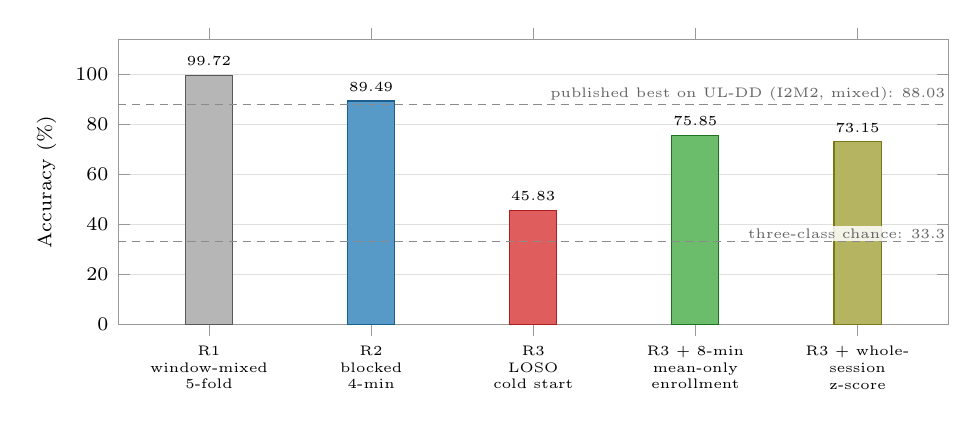
\begin{tikzpicture}
\begin{axis}[wechart, width=\columnwidth, height=5.2cm,
  ybar, bar width=17pt,
  symbolic x coords={R1,R2,R3,R3e,R3w}, xtick={R1,R2,R3,R3e,R3w},
  xticklabels={{\rone\\window-mixed\\5-fold},{\rtwo\\blocked\\4-min},{\rthree\\LOSO\\cold start},{\rthree{} + 8-min\\mean-only\\enrollment},{\rthree{} + whole-\\session\\z-score}},
  xticklabel style={font=\tiny,align=center},
  ymin=0, ymax=114, ylabel={Accuracy (\%)}, ytick={0,20,40,60,80,100},
  nodes near coords, nodes near coords style={font=\tiny\bfseries},
  enlarge x limits=0.14, clip=false]
\addplot[fill=weGray!50,  draw=weGray!80!black,  bar shift=0pt] coordinates {(R1,99.72)};
\addplot[fill=weBlue!75,  draw=weBlue!80!black,  bar shift=0pt] coordinates {(R2,89.49)};
\addplot[fill=weRed!75,   draw=weRed!80!black,   bar shift=0pt] coordinates {(R3,45.83)};
\addplot[fill=weGreen!70, draw=weGreen!70!black, bar shift=0pt] coordinates {(R3e,75.85)};
\addplot[fill=weOlive!70, draw=weOlive!80!black, bar shift=0pt] coordinates {(R3w,73.15)};
\pgfplotsextra{%
\draw[densely dashed, weGray!80] ({rel axis cs:0,0}|-{axis cs:R1,88.03}) -- ({rel axis cs:1,0}|-{axis cs:R1,88.03})
  node[pos=1, anchor=south east, font=\tiny, text=weGray!90!black, fill=white, fill opacity=0.85, text opacity=1, inner sep=1pt] {published best on UL-DD (I2M2, mixed): 88.03};
\draw[densely dashed, weGray!80] ({rel axis cs:0,0}|-{axis cs:R1,33.3}) -- ({rel axis cs:1,0}|-{axis cs:R1,33.3})
  node[pos=1, anchor=south east, font=\tiny, text=weGray!90!black, fill=white, fill opacity=0.85, text opacity=1, inner sep=1pt] {three-class chance: 33.3};}
\end{axis}
\end{tikzpicture}
\caption{The protocol ladder for LightGBM on identical features. The base
paper's best published result (I2M2, 88.03\%)~\cite{bodaghi2026uldd} and
three-class chance are marked. The deployable eight-minute enrollment exceeds
the transductive whole-session z-score. Colours follow Fig.~\ref{fig:arch}(b).}
\label{fig:ladder}
\end{figure}

Table~\ref{tab:ladder} and Fig.~\ref{fig:ladder} then hold the model and
feature set fixed and vary only the regime. Accuracy spans 54\pp{} between the
window-mixed and cold-start LOSO settings. The cold-start figure must be read
against the class distribution. Over the evaluable subjects, 25.4\% of
windows are Low (3{,}871), 33.5\% Medium (5{,}109) and 41.1\% High (6{,}257),
for 15{,}237 scored windows over the 16 evaluable drivers. A trivial rule that predicts the majority
class of the training pool (always High) scores 31.7\% averaged over drivers,
the same averaging used for every other accuracy, while the pooled High
prevalence is 41.1\%. The uncalibrated model therefore sits about 15\pp{}
above the trivial rule and 5\pp{} above the pooled prior. Eight minutes of mean-only enrollment recover the
unseen-driver figure to 75.85\%, which is above the transductive
whole-session z-score (73.15\%), and balanced accuracy rises from 44.4\% to
75.4\%. The published UL-DD results sit inside the leaky band of this ladder.

\begin{table}[!t]
\caption{Leakage controls, LightGBM, accuracy in \%. Permuted labels are
re-assigned per (subject, session, 4-minute block). Driver identity is a
19-way task with 5.3\% chance.}
\label{tab:controls}
\centering\footnotesize
\begin{tabular}{@{}lcc@{}}
\toprule
Target / labels & \rone{} window-mixed & \rtwo{} blocked \\
\midrule
Drowsiness, true labels            & 99.76 & 89.51 \\
Drowsiness, labels permuted per block & 98.68 & 36.57 \\
Driver identity (19-way)           & 99.96 & 99.34 \\
\bottomrule
\end{tabular}
\end{table}

\begin{figure}[!t]
\centering
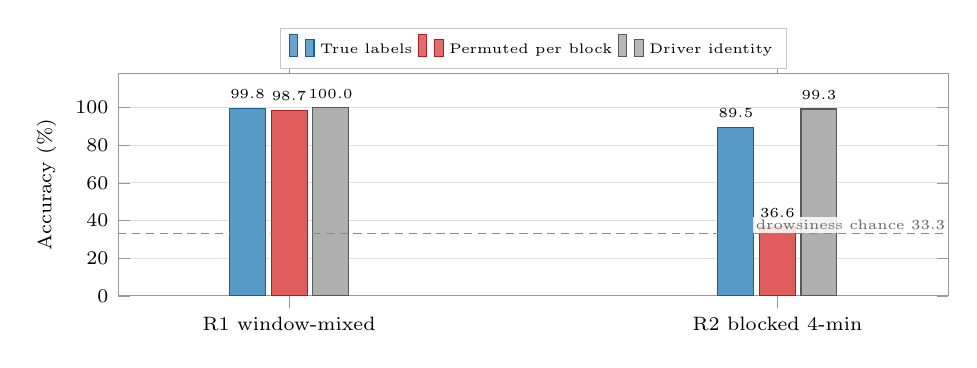
\begin{tikzpicture}
\begin{axis}[wechart, width=\columnwidth, height=4.4cm,
  ybar, bar width=13pt,
  symbolic x coords={R1,R2}, xtick={R1,R2},
  xticklabels={{\rone{} window-mixed},{\rtwo{} blocked 4-min}},
  xticklabel style={font=\scriptsize},
  ymin=0, ymax=118, ylabel={Accuracy (\%)}, ytick={0,20,40,60,80,100},
  enlarge x limits=0.35,
  legend columns=3, legend style={at={(0.5,1.02)}, anchor=south},
  nodes near coords, nodes near coords style={font=\tiny,
    /pgf/number format/precision=1, /pgf/number format/fixed, /pgf/number format/fixed zerofill}]
\addplot[fill=weBlue!75, draw=weBlue!80!black]  coordinates {(R1,99.76) (R2,89.51)};
\addplot[fill=weRed!75,  draw=weRed!80!black]   coordinates {(R1,98.68) (R2,36.57)};
\addplot[fill=weGray!55, draw=weGray!80!black]  coordinates {(R1,99.96) (R2,99.34)};
\legend{True labels, Permuted per block, Driver identity}
\pgfplotsextra{%
\draw[densely dashed, weGray!80] ({rel axis cs:0,0}|-{axis cs:R1,33.3}) -- ({rel axis cs:1,0}|-{axis cs:R1,33.3})
  node[pos=1, anchor=south east, font=\tiny, text=weGray!90!black, fill=white, fill opacity=0.85, text opacity=1, inner sep=1pt] {drowsiness chance 33.3};}
\end{axis}
\end{tikzpicture}
\caption{Leakage controls (Table~\ref{tab:controls}). Block-permuted labels
survive window-mixed evaluation and fall to chance under blocked folds. A
single 10-s window identifies the driver under either protocol.}
\label{fig:controls}
\end{figure}

The controls in Table~\ref{tab:controls} and Fig.~\ref{fig:controls} identify
the mechanism directly. With labels randomly permuted per 4-minute block, the
model still scores 98.68\% under \rone{} (99.76\% with true labels). Under
\rtwo{} the same permutation falls to chance. A single 10-s window identifies
the driver among nineteen with 99.96\% accuracy under \rone{} and 99.34\% under
\rtwo{} (chance 5.3\%). Any subject-mixed protocol therefore also rewards
recognizing who is driving.

\subsection{Architectures Across Regimes}
\label{sec:archs}
\begin{table*}[!t]
\caption{Six architectures across regimes, accuracy \% (macro-F1 \%). All
values come from the V2 experiment runner on the identical 135-d feature table
and byte-identical folds. The calibrated columns apply the same transform to
every model. n/a: configuration not run. In the mean-only column the four neural architectures are reported as mean $\pm$ seed standard deviation over three seeds; LightGBM is deterministic under this configuration (identical to four decimals across seeds).}
\label{tab:archs}
\centering\footnotesize
\begin{tabular}{@{}lccccc@{}}
\toprule
Model & \rone{} window-mixed & \rtwo{} blocked & \rthree{} + whole-session z & \rthree{} uncalibrated & \rthree{} + 8-min mean-only \\
\midrule
Graph-transformer (FatigueNet-style)~\cite{zendehbad2025fatiguenet} & 92.05 (92.03) & 70.60 (70.65) & 46.04 (41.93) & n/a & n/a \\
Pruned GNN (graph removed)      & 99.60 (99.60) & 84.65 (84.89) & 55.52 (49.64) & n/a & 57.26 $\pm$ 0.74 (50.31) \\
I2M2~\cite{madaan2024i2m2}       & 96.04 (96.17) & 84.70 (85.09) & 57.84 (51.16) & 48.80 (37.31) & 59.81 $\pm$ 0.90 (53.35) \\
Temporal transformer            & 99.51 (99.51) & 84.08 (84.22) & 47.42 (42.35) & n/a & 54.69 $\pm$ 1.80 (47.13) \\
Stacked ensemble                & 99.47 (99.47) & 88.03 (88.27) & 58.78 (50.75) & n/a & 55.84 $\pm$ 0.26 (51.53) \\
LightGBM (\sysname)             & \textbf{99.72} (99.72) & \textbf{89.49} (89.54) & \textbf{73.69} (64.97) & 45.83 (36.66) & \textbf{74.71} (68.42) \\
\bottomrule
\end{tabular}
\end{table*}

\begin{figure}[!t]
\centering
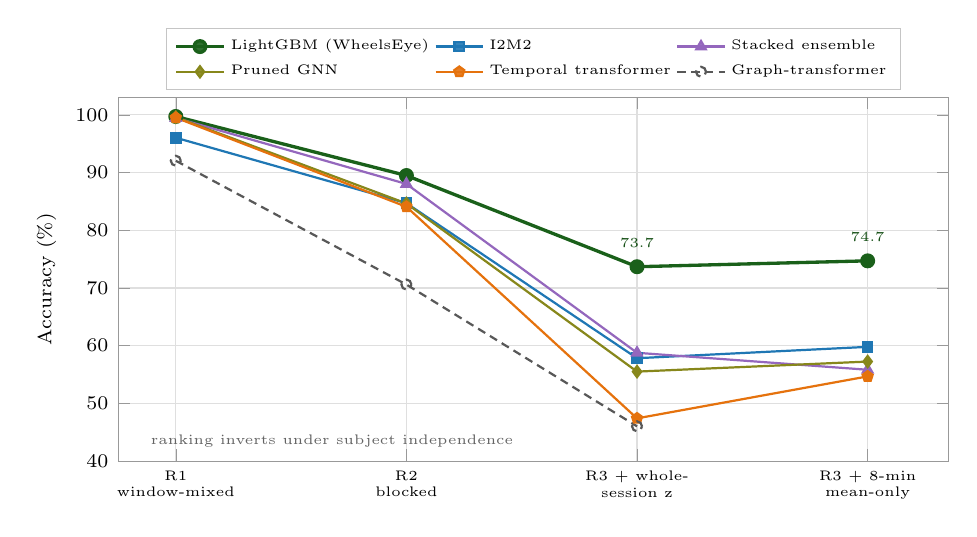
\begin{tikzpicture}
\begin{axis}[wechart, width=\columnwidth, height=6.2cm,
  xmin=0.75, xmax=4.35, ymin=40, ymax=103,
  xtick={1,2,3,4},
  xticklabels={{\rone\\window-mixed},{\rtwo\\blocked},{\rthree{} + whole-\\session z},{\rthree{} + 8-min\\mean-only}},
  xticklabel style={font=\tiny,align=center},
  ylabel={Accuracy (\%)}, ytick={40,50,60,70,80,90,100},
  xmajorgrids, grid style={weGray!22},
  legend style={at={(0.5,1.02)}, anchor=south, font=\tiny}, legend columns=3,
  legend cell align=left, clip=false]
\addplot[weGreen!60!black, very thick, mark=*, mark size=2.1pt] coordinates {(1,99.72) (2,89.49) (3,73.69) (4,74.71)};
\addplot[weBlue, thick, mark=square*, mark size=1.7pt] coordinates {(1,96.04) (2,84.70) (3,57.84) (4,59.81)};
\addplot[wePurple, thick, mark=triangle*, mark size=2.0pt] coordinates {(1,99.47) (2,88.03) (3,58.78) (4,55.84)};
\addplot[weOlive!90!black, thick, mark=diamond*, mark size=2.0pt] coordinates {(1,99.60) (2,84.65) (3,55.52) (4,57.26)};
\addplot[weOrange!90!black, thick, mark=pentagon*, mark size=1.9pt] coordinates {(1,99.51) (2,84.08) (3,47.42) (4,54.69)};
\addplot[weGray!80!black, thick, densely dashed, mark=o, mark size=1.8pt] coordinates {(1,92.05) (2,70.60) (3,46.04)};
\legend{LightGBM (\sysname), I2M2, Stacked ensemble, Pruned GNN, Temporal transformer, Graph-transformer}
\node[font=\tiny, anchor=south, text=weGreen!50!black] at (axis cs:3,75.3) {73.7};
\node[font=\tiny, anchor=south, text=weGreen!50!black] at (axis cs:4,76.3) {74.7};
\node[font=\tiny, anchor=west, text=weGray!90!black] at (axis cs:0.85,43.5) {ranking inverts under subject independence};
\end{axis}
\end{tikzpicture}
\caption{Architecture accuracy across evaluation regimes (V2 runner). Every
line starts near the ceiling under window-mixed evaluation and fans out under
subject independence, where the lightweight model leads and the
graph-transformer trails. The uncalibrated \rthree{} column and macro-F1
values are in Table~\ref{tab:archs}.}
\label{fig:regimes}
\end{figure}

Table~\ref{tab:archs} and Fig.~\ref{fig:regimes} compare the six
architectures on the V2 runner. Under \rone{} every model except the
graph-transformer saturates above 96\%, so the regime cannot rank them. Under
\rtwo{} the spread opens moderately, with LightGBM and the stacked ensemble in
front. Under \rthree{} the ranking inverts. With identical whole-session
z-scoring, LightGBM leads every fusion architecture. Under identical 8-minute
mean-only enrollment the margin widens. Relative to their whole-session
z-score results, mean subtraction moves I2M2 by $+1.9$\pp, the pruned GNN by
$+2.5$\pp{} and the stacked ensemble by $-2.9$\pp, while LightGBM gains about
ten points over its own 8-minute z-score result (Table~\ref{tab:variants}).
Without calibration, the models evaluated in that setting fall into the 46 to
49\% band that all fusion architectures had reached on the V1 pipeline.
Under matched 8-minute mean-only enrollment, with every model receiving the
identical calibrated features, LightGBM reaches 74.71\% against $59.81 \pm 0.90$\%
for I2M2, $57.26 \pm 0.74$\% for the pruned GNN, $55.84 \pm 0.26$\% for the
stacked ensemble and $54.69 \pm 1.80$\% for the transformer over three seeds each
(Table~\ref{tab:archs}); the corresponding margins are $+14.90$, $+17.45$,
$+18.87$ and $+20.02$\pp{}. Seed dispersion is one to two orders of magnitude
below every margin, so the ordering does not depend on initialisation: the largest
seed standard deviation (1.80\pp{} for the transformer) is an eighth of the
smallest margin. Architecture rankings are therefore regime-dependent,
and only the subject-independent ranking matters for deployment.

\subsection{Calibration Variants and Enrollment Length}
\label{sec:variants}
\begin{table}[!t]
\caption{Calibration variants and baselines, LightGBM, LOSO, standalone
pipeline, sensor features calibrated.}
\label{tab:variants}
\centering\footnotesize
\begin{tabular}{@{}lccl@{}}
\toprule
Variant & Acc \% & F1 \% & Nature \\
\midrule
None                              & 47.48 & 37.40 & none \\
Enrollment 8 min, z-score         & 66.03 & 59.12 & deployable \\
Enrollment 8 min, mean-only       & \textbf{75.85} & \textbf{69.65} & deployable \\
Whole alert session, z-score      & 73.15 & 64.96 & transductive \\
Whole alert session, mean-only    & 72.37 & 64.73 & transductive \\
Both sessions, mean-only          & 54.62 & 49.12 & transductive \\
CORAL (test-time alignment)~\cite{sun2016coral} & 43.01 & 38.50 & transductive \\
Supervised labelled enrollment (bound) & 80.79 & 63.97 & uses labels \\
\bottomrule
\end{tabular}
\end{table}

Table~\ref{tab:variants} compares transforms and baselines. Mean subtraction
at eight minutes leads. Z-scoring the same enrollment forfeits $9.81$\pp{}
($p=0.025$), and both whole-session variants trail the brief enrollment
($p\ge0.38$). The transductive baselines are worse still. Standardizing on
all of the driver's unlabelled windows from both sessions loses a further
twenty points, and CORAL falls below no calibration at all. Supervised
labelled enrollment buys $4.94$\pp{} of accuracy over the label-free transform
($p=0.19$, n.s.) at a cost in macro-F1.

\begin{table}[!t]
\caption{Enrollment curve, LightGBM, LOSO, standalone pipeline. Accuracy \%
(macro-F1 \%) for both transforms, and mean-only per-class recall
(Low\,/\,Medium\,/\,High).}
\label{tab:enroll}
\centering\footnotesize
\setlength{\tabcolsep}{3.5pt}
\begin{tabular}{@{}lccc@{}}
\toprule
Enrollment & Mean-only & Z-score & Recall L/M/H \\
\midrule
1 min  & 70.66 (65.39) & 58.26 (54.26) & 69.9 / 52.9 / 85.8 \\
2 min  & 74.47 (69.01) & 59.83 (53.77) & 76.8 / 59.7 / 85.2 \\
4 min  & \textbf{76.51} (70.83) & 63.16 (56.24) & 82.9 / 59.6 / 86.6 \\
8 min  & 75.85 (69.65) & 65.67 (58.94) & 79.3 / 59.6 / 87.2 \\
12 min & 71.80 (65.34) & 62.31 (55.20) & 69.4 / 56.3 / 86.2 \\
20 min & 71.58 (64.24) & 64.33 (57.60) & 73.6 / 52.3 / 86.3 \\
30 min & 73.64 (66.39) & 71.72 (65.16) & 71.0 / 61.7 / 85.1 \\
38 min & 71.53 (63.80) & 68.27 (58.65) & 68.3 / 61.8 / 81.6 \\
whole session & 72.37 (64.73) & 73.15 (64.96) & 70.4 / 60.4 / 83.4 \\
\bottomrule
\end{tabular}
\end{table}

\begin{figure}[!t]
\centering
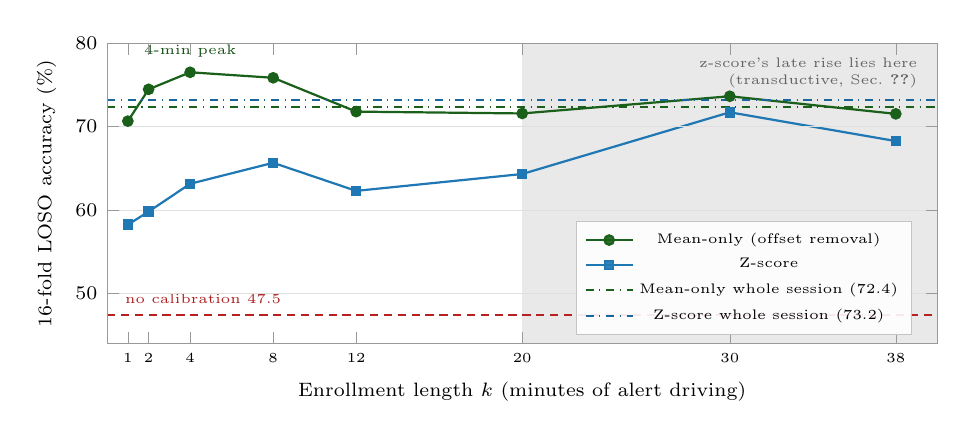
\begin{tikzpicture}
\begin{axis}[wechart, width=\columnwidth, height=5.4cm,
  xmin=0, xmax=40, ymin=44, ymax=80,
  xtick={1,2,4,8,12,20,30,38}, xticklabel style={font=\tiny},
  xlabel={Enrollment length $k$ (minutes of alert driving)},
  ylabel={16-fold LOSO accuracy (\%)},
  legend pos=south east, axis on top, clip=false]
\fill[weGray!15] (axis cs:20,44) rectangle (axis cs:40,80);
\node[font=\tiny, align=right, anchor=north east, text=weGray!90!black] at (axis cs:39.5,79.4)
  {z-score's late rise lies here\\(transductive, Sec.~\ref{sec:transductive})};
\addplot[forget plot, weRed!85!black, densely dashed, thick] coordinates {(0,47.48) (40,47.48)};
\node[font=\tiny, anchor=south west, text=weRed!80!black] at (axis cs:0.4,47.7) {no calibration 47.5};
\addplot[weGreen!60!black, thick, mark=*, mark size=1.7pt]
  coordinates {(1,70.66) (2,74.47) (4,76.51) (8,75.85) (12,71.80) (20,71.58) (30,73.64) (38,71.53)};
\addplot[weBlue, thick, mark=square*, mark size=1.5pt]
  coordinates {(1,58.26) (2,59.83) (4,63.16) (8,65.67) (12,62.31) (20,64.33) (30,71.72) (38,68.27)};
\addplot[weGreen!60!black, dashdotted, thick] coordinates {(0,72.37) (40,72.37)};
\addplot[weBlue!85!black, dashdotted, thick] coordinates {(0,73.15) (40,73.15)};
\legend{Mean-only (offset removal), Z-score, Mean-only whole session (72.4), Z-score whole session (73.2)}
\node[font=\tiny, anchor=south, text=weGreen!50!black] at (axis cs:4,77.1) {4-min peak};
\end{axis}
\end{tikzpicture}
\caption{Accuracy against enrollment length for both transforms (LightGBM,
LOSO, standalone pipeline). Mean subtraction peaks at four minutes and declines
for longer baselines, and the whole-session variant is worse than a brief
enrollment. Z-scoring plateaus and climbs only inside the shaded region, where
the baseline overlaps most of the scored alert session. Dash-dotted lines mark
the whole-session variants.}
\label{fig:enroll}
\end{figure}

Table~\ref{tab:enroll} and Fig.~\ref{fig:enroll} sweep the enrollment length
for both transforms. Mean-only peaks at four minutes (one KSS interval),
holds at eight, and \emph{declines} for longer baselines and for the whole
session. The difference between four and eight minutes lies well inside the
fold dispersion of 12 to 15\pp{} (standard error of the mean about
3.5\pp). Z-scoring instead plateaus near 64\% and climbs only inside the
shaded region, where the baseline covers most of the scored session. This is
the transductive signature analysed in Sec.~\ref{sec:transductive}.

Excluding the held-out driver's 96 enrollment windows from scoring changes
UL-DD accuracy by $-0.02$\pp{} for mean-only (75.87\% when excluded,
$p=0.67$) and by $+0.69$\pp{} for z-scoring ($p=0.38$). Macro-F1 falls from
69.65\% to 63.72\% because the excluded windows are all alert-class and the
test set rebalances. With 96 of roughly 950 windows per driver enrolled, the
shortcut is worth nothing measurable on this dataset.

\subsection{Modality Attribution}
\begin{table}[!t]
\caption{Modality lattice, LightGBM, LOSO, 8-min mean-only enrollment,
standalone pipeline. Alone, With and W/out are accuracies in \%. $\Delta$ is
the mean accuracy over the 32 subsets containing the group minus the mean over
the 31 that do not.}
\label{tab:lattice}
\centering\footnotesize
\setlength{\tabcolsep}{3pt}
\begin{tabular}{@{}lcccc@{}}
\toprule
Group (features) & Alone & With & W/out & $\Delta$ (pp) \\
\midrule
Facial action units (66)      & 63.63 & 61.84 & 48.01 & $+13.83$ \\
Autonomic: EDA, temp.\ (11)   & 47.54 & 56.93 & 52.92 & $+4.02$ \\
Posture landmarks (7)         & 44.05 & 55.74 & 54.10 & $+1.64$ \\
Face geometry (17)            & 43.42 & 55.68 & 54.16 & $+1.52$ \\
Cardiac: HR, HRV (12)         & 36.47 & 54.56 & 55.29 & $-0.73$ \\
Grip / motion (9)             & 37.87 & 53.94 & 55.91 & $-1.97$ \\
\bottomrule
\end{tabular}
\end{table}

Table~\ref{tab:lattice} reports the $2^{6}$ lattice under mean-only
enrollment. Facial action units carry the largest marginal contribution and
are the strongest single group. Autonomic signals form a second layer. Posture
and face geometry add little, and cardiac and grip contribute nothing.
Vision-only exceeds biometric-only (62.26\% against 52.44\%), and all six
sensor groups together reach only 62.49\%. The 13 drift-context features add
a further $+13.36$\pp{} on top of them ($p=0.0003$, 15 of 16 folds), a
contribution that the time-on-task control of Sec.~\ref{sec:controls2} shows
to be reproducible by elapsed drive time, and which brings the full
configuration to its headline value, $+23.41$\pp{} over
biometric-only ($p=0.002$) and $+13.59$\pp{} over vision-only ($p=0.006$).
Under z-scoring the ranking differed sharply. The action-unit marginal fell to
zero and cardiac-alone dropped below chance (32.75\%), so the z variant was
destroying signal rather than revealing modality value.

\subsection{Where Calibration Acts}
\label{sec:classes}
\begin{figure}[!t]
\centering
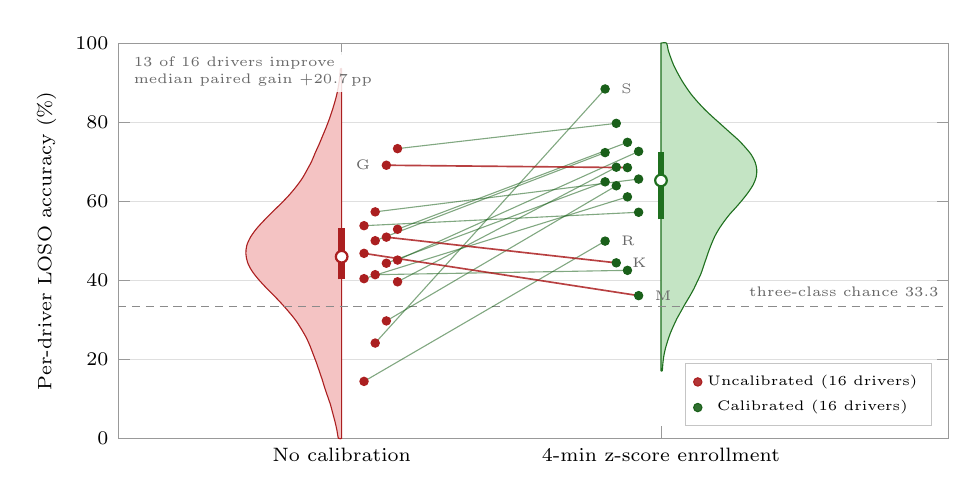
\begin{tikzpicture}
\begin{axis}[wechart, width=\columnwidth, height=6.6cm,
  xmin=0.30, xmax=2.90, ymin=0, ymax=100,
  xtick={1,2}, xticklabels={{No calibration},{4-min z-score enrollment}},
  xticklabel style={font=\scriptsize},
  ylabel={Per-driver LOSO accuracy (\%)}, ytick={0,20,40,60,80,100},
  legend style={at={(0.98,0.03)}, anchor=south east}, clip=false]
% half violins (kernel density of 16 held-out drivers)
\fill[weRed!28, draw=weRed!80!black, thin] plot[smooth] coordinates {(axis cs:1.000,0.00) (axis cs:0.990,0.00) (axis cs:0.985,2.12) (axis cs:0.979,4.25) (axis cs:0.972,6.37) (axis cs:0.965,8.50) (axis cs:0.956,10.62) (axis cs:0.947,12.74) (axis cs:0.939,14.87) (axis cs:0.930,16.99) (axis cs:0.921,19.12) (axis cs:0.911,21.24) (axis cs:0.901,23.36) (axis cs:0.889,25.49) (axis cs:0.874,27.61) (axis cs:0.857,29.74) (axis cs:0.836,31.86) (axis cs:0.813,33.98) (axis cs:0.788,36.11) (axis cs:0.762,38.23) (axis cs:0.738,40.36) (axis cs:0.718,42.48) (axis cs:0.705,44.60) (axis cs:0.700,46.73) (axis cs:0.703,48.85) (axis cs:0.715,50.97) (axis cs:0.734,53.10) (axis cs:0.758,55.22) (axis cs:0.784,57.35) (axis cs:0.811,59.47) (axis cs:0.836,61.59) (axis cs:0.858,63.72) (axis cs:0.877,65.84) (axis cs:0.892,67.97) (axis cs:0.906,70.09) (axis cs:0.917,72.21) (axis cs:0.929,74.34) (axis cs:0.940,76.46) (axis cs:0.951,78.59) (axis cs:0.961,80.71) (axis cs:0.970,82.83) (axis cs:0.978,84.96) (axis cs:0.985,87.08) (axis cs:0.990,89.21) (axis cs:0.994,91.33) (axis cs:0.996,93.45) (axis cs:1.000,93.45)} -- cycle;
\fill[weGreen!28, draw=weGreen!70!black, thin] plot[smooth] coordinates {(axis cs:2.000,17.11) (axis cs:2.004,17.11) (axis cs:2.006,18.99) (axis cs:2.009,20.88) (axis cs:2.014,22.76) (axis cs:2.021,24.65) (axis cs:2.029,26.53) (axis cs:2.039,28.41) (axis cs:2.050,30.30) (axis cs:2.063,32.18) (axis cs:2.076,34.06) (axis cs:2.090,35.95) (axis cs:2.103,37.83) (axis cs:2.114,39.72) (axis cs:2.125,41.60) (axis cs:2.133,43.48) (axis cs:2.141,45.37) (axis cs:2.149,47.25) (axis cs:2.158,49.14) (axis cs:2.168,51.02) (axis cs:2.181,52.90) (axis cs:2.197,54.79) (axis cs:2.215,56.67) (axis cs:2.236,58.55) (axis cs:2.256,60.44) (axis cs:2.274,62.32) (axis cs:2.289,64.21) (axis cs:2.298,66.09) (axis cs:2.300,67.97) (axis cs:2.295,69.86) (axis cs:2.283,71.74) (axis cs:2.264,73.63) (axis cs:2.242,75.51) (axis cs:2.216,77.39) (axis cs:2.190,79.28) (axis cs:2.164,81.16) (axis cs:2.139,83.05) (axis cs:2.117,84.93) (axis cs:2.097,86.81) (axis cs:2.080,88.70) (axis cs:2.065,90.58) (axis cs:2.052,92.46) (axis cs:2.040,94.35) (axis cs:2.031,96.23) (axis cs:2.023,98.12) (axis cs:2.017,100.00) (axis cs:2.000,100.00)} -- cycle;
% chance
\draw[densely dashed, weGray!80] (axis cs:0.30,33.3) -- (axis cs:2.90,33.3)
  node[pos=1, anchor=south east, font=\tiny, text=weGray!90!black] {three-class chance 33.3};
% paired slope lines
\addplot[weGreen!60!black, opacity=0.55, thin, forget plot] coordinates {(1.070,14.4) (1.825,49.9)};
\addplot[weGreen!60!black, opacity=0.55, thin, forget plot] coordinates {(1.105,24.1) (1.825,88.4)};
\addplot[weGreen!60!black, opacity=0.55, thin, forget plot] coordinates {(1.140,29.7) (1.860,63.9)};
\addplot[weGreen!60!black, opacity=0.55, thin, forget plot] coordinates {(1.175,39.6) (1.860,68.6)};
\addplot[weGreen!60!black, opacity=0.55, thin, forget plot] coordinates {(1.070,40.4) (1.895,61.1)};
\addplot[weGreen!60!black, opacity=0.55, thin, forget plot] coordinates {(1.105,41.4) (1.895,42.5)};
\addplot[weGreen!60!black, opacity=0.55, thin, forget plot] coordinates {(1.140,44.3) (1.825,64.9)};
\addplot[weGreen!60!black, opacity=0.55, thin, forget plot] coordinates {(1.175,45.1) (1.930,72.6)};
\addplot[weRed!80!black, opacity=0.85, semithick, forget plot] coordinates {(1.070,46.8) (1.930,36.1)};
\addplot[weGreen!60!black, opacity=0.55, thin, forget plot] coordinates {(1.105,50.0) (1.825,72.3)};
\addplot[weRed!80!black, opacity=0.85, semithick, forget plot] coordinates {(1.140,50.9) (1.860,44.4)};
\addplot[weGreen!60!black, opacity=0.55, thin, forget plot] coordinates {(1.175,52.9) (1.895,74.9)};
\addplot[weGreen!60!black, opacity=0.55, thin, forget plot] coordinates {(1.070,53.8) (1.930,57.2)};
\addplot[weGreen!60!black, opacity=0.55, thin, forget plot] coordinates {(1.105,57.3) (1.930,65.6)};
\addplot[weRed!80!black, opacity=0.85, semithick, forget plot] coordinates {(1.140,69.1) (1.895,68.5)};
\addplot[weGreen!60!black, opacity=0.55, thin, forget plot] coordinates {(1.175,73.3) (1.860,79.7)};
% interquartile bars and medians
\addplot[weRed!80!black, line width=2.4pt, forget plot] coordinates {(1,40.20) (1,53.12)};
\addplot[weGreen!70!black, line width=2.4pt, forget plot] coordinates {(2,55.38) (2,72.38)};
\addplot[only marks, mark=*, mark size=2.1pt, mark options={fill=white, draw=weRed!80!black, line width=0.8pt}, forget plot] coordinates {(1,45.95)};
\addplot[only marks, mark=*, mark size=2.1pt, mark options={fill=white, draw=weGreen!70!black, line width=0.8pt}, forget plot] coordinates {(2,65.25)};
% driver points
\addplot[only marks, mark=*, mark size=1.5pt, weRed!80!black] coordinates {(1.070,14.4) (1.105,24.1) (1.140,29.7) (1.175,39.6) (1.070,40.4) (1.105,41.4) (1.140,44.3) (1.175,45.1) (1.070,46.8) (1.105,50.0) (1.140,50.9) (1.175,52.9) (1.070,53.8) (1.105,57.3) (1.140,69.1) (1.175,73.3)};
\addplot[only marks, mark=*, mark size=1.5pt, weGreen!60!black] coordinates {(1.825,49.9) (1.825,88.4) (1.860,63.9) (1.860,68.6) (1.895,61.1) (1.895,42.5) (1.825,64.9) (1.930,72.6) (1.930,36.1) (1.825,72.3) (1.860,44.4) (1.895,74.9) (1.930,57.2) (1.930,65.6) (1.895,68.5) (1.860,79.7)};
\legend{Uncalibrated (16 drivers), Calibrated (16 drivers)}
\node[font=\tiny, anchor=west, text=weGray!95!black] at (axis cs:1.845,88.4) {S};
\node[font=\tiny, anchor=west, text=weGray!95!black] at (axis cs:1.845,49.9) {R};
\node[font=\tiny, anchor=west, text=weGray!95!black] at (axis cs:1.880,44.4) {K};
\node[font=\tiny, anchor=west, text=weGray!95!black] at (axis cs:1.950,36.1) {M};
\node[font=\tiny, anchor=east, text=weGray!95!black] at (axis cs:1.120,69.1) {G};
\node[font=\tiny, align=left, anchor=north west, text=weGray!95!black, fill=white, fill opacity=0.85, text opacity=1, inner sep=2pt] at (axis cs:0.33,98)
  {13 of 16 drivers improve\\median paired gain $+20.7$\,pp};
\end{axis}
\end{tikzpicture}
\caption{Per-driver LOSO accuracy on UL-DD without calibration and with
four-minute z-score enrollment (LightGBM). Half violins show the kernel
density over the 16 held-out drivers, the thick bar and open circle mark the
interquartile range and median, and each thin line connects the two scores of
one driver (green rises, red falls). Points are jittered horizontally for
visibility. Exact values are in Table~\ref{tab:drivers}.}
\label{fig:drivers}
\end{figure}

\begin{table}[!t]
\caption{Per-subject LOSO accuracy \%, LightGBM, z-score 4-min enrollment
(16 evaluable subjects). The uncalibrated column comes from the V2 runner and
the calibrated column from the standalone pipeline (Sec.~\ref{sec:calibration}).}
\label{tab:drivers}
\centering\footnotesize
\setlength{\tabcolsep}{4pt}
\begin{tabular}{@{}lccc@{\hspace{12pt}}lccc@{}}
\toprule
Subj. & Uncal. & 4-min & $\Delta$ & Subj. & Uncal. & 4-min & $\Delta$ \\
\midrule
A & 41.4 & 42.5 & $+1.1$  & K & 50.9 & 44.4 & $-6.6$  \\
B & 53.8 & 57.2 & $+3.5$  & M & 46.8 & 36.1 & $-10.7$ \\
D & 52.9 & 74.9 & $+22.0$ & N & 44.3 & 64.9 & $+20.6$ \\
E & 45.1 & 72.6 & $+27.5$ & O & 40.4 & 61.1 & $+20.7$ \\
G & 69.1 & 68.5 & $-0.6$  & P & 39.6 & 68.6 & $+29.0$ \\
H & 73.3 & 79.7 & $+6.4$  & Q & 29.7 & 63.9 & $+34.2$ \\
I & 50.0 & 72.3 & $+22.3$ & R & 14.4 & 49.9 & $+35.5$ \\
J & 57.3 & 65.6 & $+8.3$  & S & 24.1 & 88.4 & $+64.3$ \\
\midrule
\multicolumn{4}{@{}l}{Mean over subjects} & & 45.8 & 63.2 & $+17.3$ \\
\bottomrule
\end{tabular}
\end{table}

\begin{table}[!t]
\caption{Pooled per-class recall \% and ordinal errors, LightGBM, LOSO,
standalone pipeline. The I2M2 row comes from the V2 runner. MAE is in ordinal
class steps. 2-step counts Low$\leftrightarrow$High confusions.}
\label{tab:classes}
\centering\footnotesize
\setlength{\tabcolsep}{4pt}
\begin{tabular}{@{}lccccc@{}}
\toprule
Configuration & Low & Med. & High & MAE & 2-step \% \\
\midrule
No calibration              & 19.4 & 55.1 & 58.6 & 0.701 & 17.56 \\
Z-score, 8-min enrollment   & 68.0 & 52.8 & 75.7 & 0.370 & 3.08 \\
Z-score, whole session      & 76.3 & 60.6 & 81.6 & 0.268 & 0.01 \\
Mean-only, 4-min enrollment & 82.9 & 59.6 & 86.6 & \textbf{0.234} & 0.01 \\
Mean-only, 8-min enrollment & 79.3 & 59.6 & \textbf{87.2} & 0.242 & 0.11 \\
I2M2, whole-session z-score & 46.4 & 47.4 & 73.3 & 0.428 & 0.67 \\
\bottomrule
\end{tabular}
\end{table}

\begin{figure}[!t]
\centering
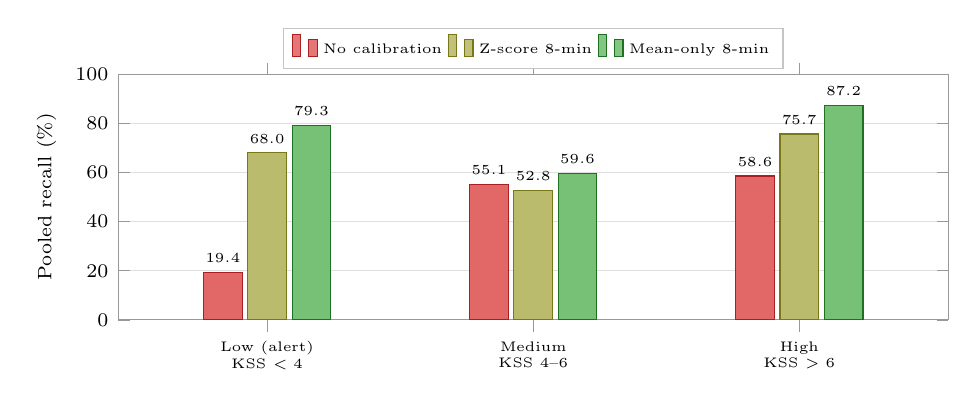
\begin{tikzpicture}
\begin{axis}[wechart, width=\columnwidth, height=4.7cm,
  ybar, bar width=14pt,
  symbolic x coords={Low,Medium,High}, xtick={Low,Medium,High},
  xticklabels={{Low (alert)\\KSS $<4$},{Medium\\KSS 4--6},{High\\KSS $>6$}},
  xticklabel style={font=\tiny,align=center},
  ymin=0, ymax=100, ylabel={Pooled recall (\%)},
  enlarge x limits=0.28,
  legend columns=3, legend style={at={(0.5,1.02)}, anchor=south},
  nodes near coords, nodes near coords style={font=\tiny,
    /pgf/number format/precision=1, /pgf/number format/fixed, /pgf/number format/fixed zerofill}]
\addplot[fill=weRed!70,   draw=weRed!80!black]   coordinates {(Low,19.4) (Medium,55.1) (High,58.6)};
\addplot[fill=weOlive!65, draw=weOlive!80!black] coordinates {(Low,68.0) (Medium,52.8) (High,75.7)};
\addplot[fill=weGreen!65, draw=weGreen!70!black] coordinates {(Low,79.3) (Medium,59.6) (High,87.2)};
\legend{No calibration, Z-score 8-min, Mean-only 8-min}
\end{axis}
\end{tikzpicture}
\caption{Pooled per-class recall before and after calibration (LightGBM,
LOSO, standalone pipeline). Mean subtraction recovers all three classes,
including the transitional Medium class. Z-scoring trades Medium for Low.}
\label{fig:classes}
\end{figure}

Fold-pooled per-class recall and ordinal errors (Table~\ref{tab:classes},
Fig.~\ref{fig:classes}) locate the gain. The uncalibrated model recognizes
under a fifth of alert windows. Z-scoring raises Low at the cost of Medium.
Mean subtraction recovers all three classes, including the transitional
Medium class, cuts the mean absolute ordinal error from 0.70 to 0.24 class
steps and nearly eliminates two-step Low-to-High confusions (17.6\% of windows
to 0.1\%). Per driver (Fig.~\ref{fig:drivers} and Table~\ref{tab:drivers}, the
four-minute z-score variant for which per-fold values were logged), 13 of the 16 improve with a
median gain of $+20.7$\pp. The hardest subjects are transformed (S rises from
24\% to 88\%), while K and M lose 6.6 to 10.7\pp{} and G is essentially flat.
Dispersion across drivers remains the dominant source of variance.
A single-pipeline rerun of the headline mean-only eight-minute configuration
reproduces the aggregate to within 0.2\pp{} (46.28\% uncalibrated, 75.70\%
calibrated with enrollment windows scored, 75.91\% with them excluded), and its
per-driver values are released with the analysis scripts.

\subsection{Replication on MePhy and RLDD}
\label{sec:replication}
\begin{table}[!t]
\caption{MePhy replication~\cite{zendehbad2025fatiguenet}. LightGBM, 19-user
leave-one-user-out, first-generation 17-feature pipeline. Baselines come from
each user's rest-condition windows.}
\label{tab:mephy}
\centering\footnotesize
\begin{tabular}{@{}lcc@{}}
\toprule
Calibration from rest windows & Acc \% & F1 \% \\
\midrule
None                              & 44.86 & 42.18 \\
First 24 rest windows, z-score    & 44.66 & 46.90 \\
First 24 rest windows, mean-only  & \textbf{51.18} & \textbf{53.72} \\
All rest windows, mean-only       & 51.17 & 53.54 \\
\bottomrule
\end{tabular}
\end{table}

On MePhy (Table~\ref{tab:mephy}), mean-only rest enrollment raises
leave-one-user-out macro-F1 by $+11.5$\pp{} (95\% CI $[+3.1,+19.8]$,
$p=0.014$) and accuracy by $+6.3$\pp{} ($p=0.16$, n.s.\ at 19 users). The
z-score variant does not help, and mean-only exceeds it ($p=0.029$). The
direction and the mean-versus-z pattern replicate. The magnitude is smaller,
which is consistent with 17 features carrying less per-subject offset than
135.

\begin{table}[!t]
\caption{RLDD replication~\cite{ghoddoosian2019uta}. LightGBM, 59 subjects,
binary alert vs.\ drowsy, LOSO. Enrollment windows are excluded from scoring.
Inflation is the accuracy gained by scoring them. Whole-session calibration
cannot be evaluated because the baseline consumes every alert window.}
\label{tab:rldd}
\centering\footnotesize
\setlength{\tabcolsep}{3.5pt}
\begin{tabular}{@{}lccccc@{}}
\toprule
Calibration & Acc \% & F1 \% & Alert rec. & Drowsy rec. & Inflation \\
\midrule
None                 & 64.01 & 61.38 & 61.5 & 66.7 & n/a \\
Mean-only, 2.5 min   & 77.56 & 75.78 & 82.6 & 73.7 & $+2.04$ \\
Mean-only, 5 min     & 79.56 & 77.88 & 85.4 & 76.7 & $+2.98$ \\
Z-score, 5 min       & \textbf{85.00} & \textbf{83.73} & \textbf{87.7} & \textbf{83.5} & $+3.68$ \\
Whole session        & \multicolumn{5}{c}{not evaluable} \\
\bottomrule
\end{tabular}
\end{table}

\begin{figure}[!t]
\centering
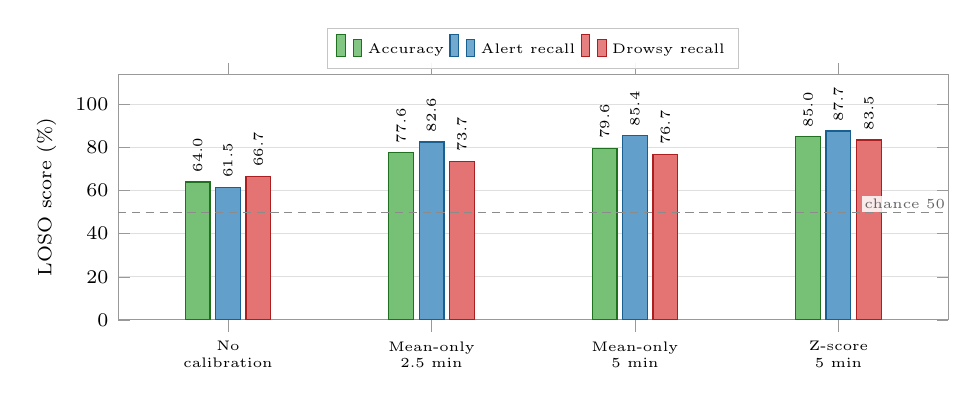
\begin{tikzpicture}
\begin{axis}[wechart, width=\columnwidth, height=4.7cm,
  ybar, bar width=9pt,
  symbolic x coords={None,M25,M5,Z5}, xtick={None,M25,M5,Z5},
  xticklabels={{No\\calibration},{Mean-only\\2.5 min},{Mean-only\\5 min},{Z-score\\5 min}},
  xticklabel style={font=\tiny,align=center},
  ymin=0, ymax=114, ytick={0,20,40,60,80,100}, ylabel={LOSO score (\%)},
  enlarge x limits=0.18,
  legend columns=3, legend style={at={(0.5,1.02)}, anchor=south},
  nodes near coords, nodes near coords style={font=\tiny, rotate=90, anchor=west,
    /pgf/number format/precision=1, /pgf/number format/fixed, /pgf/number format/fixed zerofill}]
\addplot[fill=weGreen!65, draw=weGreen!70!black] coordinates {(None,64.01) (M25,77.56) (M5,79.56) (Z5,85.00)};
\addplot[fill=weBlue!70,  draw=weBlue!80!black]  coordinates {(None,61.5) (M25,82.6) (M5,85.4) (Z5,87.7)};
\addplot[fill=weRed!65,   draw=weRed!80!black]   coordinates {(None,66.7) (M25,73.7) (M5,76.7) (Z5,83.5)};
\legend{Accuracy, Alert recall, Drowsy recall}
\pgfplotsextra{%
\draw[densely dashed, weGray!80] ({rel axis cs:0,0}|-{axis cs:None,50}) -- ({rel axis cs:1,0}|-{axis cs:None,50})
  node[pos=1, anchor=south east, font=\tiny, text=weGray!90!black, fill=white, fill opacity=0.85, text opacity=1, inner sep=1pt] {chance 50};}
\end{axis}
\end{tikzpicture}
\caption{RLDD replication at 59 subjects with enrollment windows excluded from
scoring (LightGBM, LOSO, binary task). Accuracy and both class recalls rise
together, and z-scoring beats mean subtraction on this own-device dataset.
Exact values are in Table~\ref{tab:rldd}.}
\label{fig:rldd}
\end{figure}

On RLDD (Table~\ref{tab:rldd}, Fig.~\ref{fig:rldd}), with enrollment windows
excluded from scoring, mean-only calibration from five minutes of alert video
raises leave-one-subject-out accuracy from 64.01\% to 79.56\% ($+15.55$\pp,
95\% CI $[+10.4,+20.8]$, $p<0.0001$, 48 of 59 folds, $d_z=0.75$). Alert-class
recall rises from 61.5\% to 85.4\%, the same class-specific recovery as on
UL-DD. Two and a half minutes of enrollment already give 77.56\%. Unlike the
fixed-rig datasets, variance normalization is better here. Z-scoring the same
five-minute enrollment reaches 85.00\%, which is $+5.44$\pp{} over mean-only
($p=0.0030$, 32 of 50 decided folds).

\begin{figure}[!t]
\centering
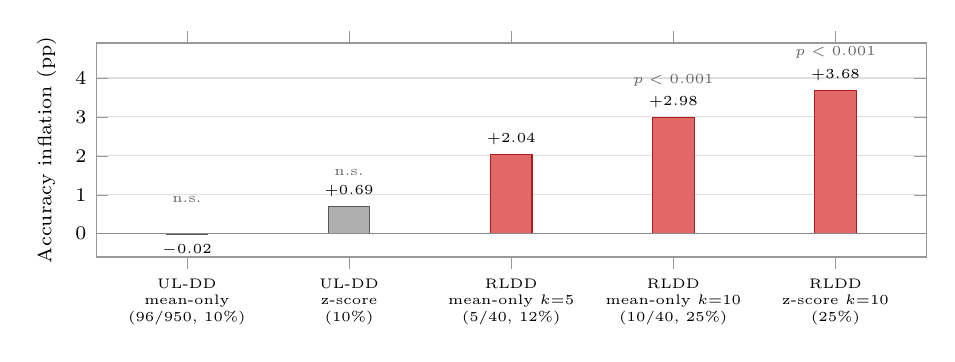
\begin{tikzpicture}
\begin{axis}[wechart, width=\columnwidth, height=4.3cm,
  ybar, bar width=15pt,
  symbolic x coords={UM,UZ,RM5,RM10,RZ10}, xtick={UM,UZ,RM5,RM10,RZ10},
  xticklabels={{UL-DD\\mean-only\\(96/950, 10\%)},{UL-DD\\z-score\\(10\%)},{RLDD\\mean-only $k{=}5$\\(5/40, 12\%)},{RLDD\\mean-only $k{=}10$\\(10/40, 25\%)},{RLDD\\z-score $k{=}10$\\(25\%)}},
  xticklabel style={font=\tiny,align=center},
  ymin=-0.6, ymax=4.9, ytick={0,1,2,3,4}, ylabel={Accuracy inflation (pp)},
  enlarge x limits=0.14, clip=false,
  nodes near coords, nodes near coords style={font=\tiny\bfseries,
    /pgf/number format/precision=2, /pgf/number format/fixed, /pgf/number format/fixed zerofill, /pgf/number format/showpos}]
\addplot[fill=weGray!55, draw=weGray!80!black, bar shift=0pt] coordinates {(UM,-0.02) (UZ,0.69)};
\addplot[fill=weRed!70,  draw=weRed!80!black,  bar shift=0pt] coordinates {(RM5,2.04) (RM10,2.98) (RZ10,3.68)};
\pgfplotsextra{%
\draw[weGray!80] ({rel axis cs:0,0}|-{axis cs:UM,0}) -- ({rel axis cs:1,0}|-{axis cs:UM,0});}
\node[font=\tiny, text=weGray!90!black, anchor=south] at (axis cs:UM,0.55) {n.s.};
\node[font=\tiny, text=weGray!90!black, anchor=south] at (axis cs:UZ,1.25) {n.s.};
\node[font=\tiny, text=weGray!90!black, anchor=south] at (axis cs:RM10,3.55) {$p<0.001$};
\node[font=\tiny, text=weGray!90!black, anchor=south] at (axis cs:RZ10,4.25) {$p<0.001$};
\end{axis}
\end{tikzpicture}
\caption{Accuracy gained by scoring the enrollment windows, against the share
of the test set they occupy. The gain is nil on UL-DD (96 of about 950
windows per driver), 2 to 4\pp{} on RLDD (12 to 25\%), and unbounded for
whole-session calibration, which leaves nothing of the alert class to score.}
\label{fig:inflation}
\end{figure}

Scoring the enrollment windows would have added 2.04, 2.98 and 3.68\pp{} to
the three calibrated RLDD configurations (Fig.~\ref{fig:inflation}). On UL-DD
the same shortcut adds nothing, because the enrollment is a tenth of each
driver's windows rather than a quarter. Whole-session calibration cannot be
evaluated on RLDD at all. The baseline consumes every alert window of every
subject and leaves nothing of that class to score.

\subsection{Time-on-Task, Session Identity and Warning-Level Controls}
\label{sec:controls2}
\begin{table}[!t]
\caption{Time-on-task, session-identity and enrollment-validity controls,
LightGBM, LOSO, 8-min mean-only enrollment unless stated. All values in \%.
Accuracy is the mean over folds. Values come from a single re-implementation of
the protocol run on the exact 135-feature list; its headline reproduces the main
pipeline to within 0.2\pp{}.}
\label{tab:controls2}
\centering\footnotesize
\setlength{\tabcolsep}{3pt}
\begin{tabular}{@{}lccc@{}}
\toprule
Configuration & Acc & Bal.\ acc & F1 \\
\midrule
Majority-class rule (training pool)               & 31.69 & 33.3 & n/a \\
Prior-matched random guessing                     & 34.56 & 33.3 & n/a \\
Sensor features only (122)                        & 63.57 & 64.56 & 62.74 \\
Sensor + drift context (full model, 135)          & 75.70 & 75.22 & 74.49 \\
Sensor + elapsed time (122 + 2)                   & 75.59 & 75.25 & 74.59 \\
Sensor + drift context, permuted in session       & 62.76 & 64.03 & 62.39 \\
Elapsed time only (2)                             & 39.53 & 33.90 & 29.02 \\
Drift context only (13)                           & 45.62 & 44.95 & 45.00 \\
\midrule
Drowsy session only, Med.\ vs.\ High, majority     & 80.01 & 50.00 & n/a \\
Drowsy session only, Med.\ vs.\ High, uncalibrated & 87.90 & 78.66 & 76.24 \\
Drowsy session only, Med.\ vs.\ High, calibrated   & 85.96 & 75.83 & 73.51 \\
Enrollment from drowsy session (wrong state)      & 6.04 & 6.43 & 5.98 \\
\bottomrule
\end{tabular}
\end{table}

Table~\ref{tab:controls2} reports the controls of Sec.~\ref{sec:regimes}.
Sensor features alone reach 63.57\% and the full model 75.70\% under mean-only
enrollment, so the thirteen drive-relative context features are worth
$+12.13$\pp{}. Two controls bound what that gain represents. Permuting the
context rows within each session destroys it entirely (62.76\%, 0.8\pp{}
\emph{below} sensor-only), which confirms that the gain depends on the temporal
ordering of those features rather than on their marginal distributions.
Replacing them with two explicit elapsed-time features, however, recovers almost
all of it (75.59\%), while elapsed time alone reaches only 39.53\% against a
prior-matched random baseline of 34.56\%. The context features are therefore not
separable from time-on-task by this experiment: they carry information that a
clock also carries, and the $+12.13$\pp{} should be read as the value of
drive-relative temporal information in general rather than as evidence for the
particular drift encoding. We regard this as a genuine capability rather than an
artifact, since time-on-task is an established fatigue driver and a deployed
system knows how long the current drive has lasted, but it does bound the claim:
the contribution is temporal, and its parameterisation is interchangeable. Drift
context alone (45.62\%) exceeds elapsed time alone by 6.1\pp{}, which is the
only evidence here that the physiological drift measures add anything beyond a
clock.

The temporal confound is a property of UL-DD's session structure rather than of
the calibration mechanism. Drowsy sessions begin at KSS $\ge 6$ and drowsiness
rises within each session, so time-into-session is label-correlated by
construction. RLDD has no such structure: each subject contributes one video per
state, labels are assigned per video rather than per window, windows do not
overlap, and no feature encodes a session-relative timestamp, so a clock cannot
predict the label. On that dataset mean-only enrollment calibration still raises
leave-one-subject-out accuracy from 64.01\% to 79.56\% with the enrollment
windows excluded from scoring ($+15.55$\pp{}, 95\% CI $+10.4$ to $+20.8$,
$p < 10^{-4}$, 48 of 59 folds), and alert-class recall from 61.5\% to 85.4\%.
The calibration mechanism is therefore established on data where the elapsed-time
explanation is unavailable, and the UL-DD temporal contribution should be read as
an additional and separable effect rather than as the basis of the result.

Inside the drowsy session, where session identity is constant and cannot inform
the decision, separating Medium from High windows reaches 87.90\% (balanced
78.66\%) without calibration and 85.96\% (balanced 75.83\%) with it, against a
within-session majority baseline of 80.01\%. Calibration therefore does
\emph{not} improve severity grading within a drowsy drive; it slightly degrades
it. Both variants exceed the majority baseline in balanced accuracy, so the model
does discriminate drowsiness levels within a single session, but the benefit of
per-driver calibration is confined to separating the alert state from the drowsy
states rather than to grading severity among them. This bounds the mechanism
claim of Sec.~\ref{sec:offsetremoval} and is consistent with the per-class
pattern of Table~\ref{tab:classes}, where calibration lifts Low and High far
more than Medium.

When the enrollment baseline is drawn from the drowsy session instead of the
alert session, accuracy collapses to 6.04\% (balanced 6.43\%; per-class recall
6.1, 10.5 and 2.7\% for Low, Medium and High), far below both the 31.69\%
majority rule and the 34.56\% random baseline. An invalid enrollment does not
merely remove the benefit of calibration, it inverts the decision boundary. This
is the strongest available evidence that the mechanism is a reference to the
driver's own alert state rather than generic per-subject normalisation, and it
defines the failure mode a deployment must prevent: enrollment has to be gated on
a genuinely alert driver.

\begin{table}[!t]
\caption{Warning-level metrics on UL-DD for the headline configuration
(LightGBM, 8-min mean-only enrollment, causal three-window majority, alarm
equals a smoothed High prediction).}
\label{tab:alarm}
\centering\footnotesize
\begin{tabular}{@{}lc@{}}
\toprule
Metric & Value \\
\midrule
False-alarm episodes per Low-labelled hour   & 1.12 \\
False-alarm episodes per alert-session hour  & 0.57 \\
Low windows under alarm (\%)                                & 0.52 \\
High windows under alarm (\%)                               & 87.31 \\
Median latency to first alarm, KSS $\ge 7$ (min) & 0.00 \\
Sessions detected within 1 / 5 min, KSS $\ge 7$ (\%) & 69 / 81 \\
Median latency to first alarm, KSS $\ge 8$ (min) & 0.00 \\
Sessions detected within 1 / 5 min, KSS $\ge 8$ (\%) & 93 / 100 \\
Drowsy sessions alarming before the first High label & 8 of 16 \\
\bottomrule
\end{tabular}
\end{table}

Table~\ref{tab:alarm} translates window predictions into warning behaviour for
the headline configuration. The system raises 0.57 false-alarm episodes per
alert-session hour, with 0.52\% of alert-labelled windows under alarm, while
covering 87.31\% of High windows; eight of sixteen drowsy sessions raise an alarm
before the first High label is recorded. For onsets at KSS $\ge 8$, 93\% of
sessions are detected within one minute and 100\% within five, which satisfies
the five-minute detection criterion of the DDAW regulation; at KSS $\ge 7$ the
figures are 69\% and 81\%. Median latency is zero at both thresholds because
UL-DD drowsy sessions begin at KSS $\ge 6$, so the alarm is frequently already
active when the threshold is crossed. Latency is therefore uninformative on this
dataset and coverage is the meaningful measure.

\subsection{Statistical Certification}
\label{sec:stats}
\begin{table*}[!t]
\caption{Paired comparisons over 16 LOSO folds, accuracy in percentage points.
CI is the 95\% bootstrap interval. W/L counts wins and losses by held-out
driver. $d_z$ is paired Cohen's $d$ and $\delta$ is Cliff's delta. n.s.\ means
not significant at $p<0.05$. Rows 1 to 9 come from the standalone pipeline and
rows 10 to 14 (architecture comparisons) from the V2 runner. The
architecture rows are paired on the seed-0 runs; the corresponding three-seed
means in Table~\ref{tab:archs} shift each margin by at most 0.8\pp{}
($+14.90$, $+18.87$, $+17.45$ and $+20.02$\pp{} respectively) without changing
any conclusion.}
\label{tab:stats}
\centering\footnotesize
\begin{tabular}{@{}lccccc@{}}
\toprule
Comparison & $\Delta$ & 95\% CI & Wilcoxon $p$ & W/L & $d_z$\,/\,$\delta$ \\
\midrule
Mean-only 8-min vs.\ no calibration            & $+28.37$ & $[+19.4,+37.6]$ & $<$0.0001 & 16/0 & 1.48 / 0.87 \\
Mean-only 8-min vs.\ z-score 8-min             & $+9.81$  & $[+2.5,+18.0]$  & 0.0250 & 12/4 & 0.60 / 0.39 \\
Mean-only 8-min vs.\ z-score whole session     & $+2.69$  & $[-4.1,+9.3]$   & 0.38 n.s. & 10/6 & 0.19 / 0.14 \\
Mean-only 8-min vs.\ I2M2 (whole-session z)    & $+18.00$ & $[+8.9,+27.4]$  & 0.0042 & 13/3 & 0.92 / 0.73 \\
Mean-only 8-min vs.\ I2M2 (uncalibrated)       & $+27.05$ & $[+14.1,+39.6]$ & 0.0010 & 14/2 & 1.00 / 0.76 \\
Mean-only 8-min vs.\ supervised labelled enrollment & $-4.94$ & $[-13.1,+2.5]$ & 0.19 n.s. & 4/12 & $-0.30$ / $-0.25$ \\
All+context vs.\ biometric-only (mean-only)    & $+23.41$ & $[+12.4,+34.7]$ & 0.0021 & 13/3 & 1.00 / 0.73 \\
All+context vs.\ vision-only (mean-only)       & $+13.59$ & $[+6.0,+20.6]$  & 0.0063 & 14/2 & 0.88 / 0.62 \\
All+context vs.\ all six without context       & $+13.36$ & $[+7.6,+19.4]$  & 0.0003 & 15/1 & 1.06 / 0.58 \\
Mean-only 8-min, both models: LightGBM vs.\ I2M2    & $+14.94$ & $[+5.4,+25.2]$  & 0.0131 & 12/4 & 0.71 / 0.59 \\
Mean-only 8-min, both models: LightGBM vs.\ stacked & $+18.83$ & $[+11.7,+26.3]$ & 0.0001 & 15/1 & 1.22 / 0.70 \\
Mean-only 8-min, both models: LightGBM vs.\ pruned GNN & $+16.66$ & $[+9.6,+24.1]$ & 0.0006 & 13/3 & 1.08 / 0.69 \\
Whole-session z: LightGBM vs.\ I2M2            & $+15.85$ & $[+9.4,+22.5]$  & 0.0006 & 14/2 & n/a \\
Whole-session z: LightGBM vs.\ graph-transformer & $+27.65$ & $[+20.6,+35.4]$ & $<$0.0001 & 16/0 & n/a \\
\bottomrule
\end{tabular}
\end{table*}

Table~\ref{tab:stats} certifies the paired comparisons with effect sizes. The
headline gain of mean-only enrollment over no calibration is $+28.37$\pp{}
(95\% CI $[+19.4,+37.6]$, $p<0.0001$, 16 of 16 drivers, $d_z=1.48$). Under
matched 8-minute enrollment, LightGBM exceeds I2M2, the stacked ensemble and
the pruned GNN in accuracy and in macro-F1 (F1 margins $+15.17$, $+16.64$ and
$+17.62$\pp, all $p\le0.013$). Under whole-session z-scoring it exceeds every
fusion architecture at $p\le0.0006$. Two comparisons are not significant even
per test, mean-only against whole-session z-scoring and supervised against
label-free enrollment. Under a Holm correction across the fourteen
comparisons, the ten with $p\le0.0063$ survive and the four with
$p\ge0.0131$ do not. The four include the mean-only margins over z-scoring and
over I2M2. The claims of this paper rest on the surviving group.

\subsection{Efficiency and Pipeline Leakage}
\label{sec:efficiency}\label{sec:leakage}
\begin{table}[!t]
\caption{Deployment-model efficiency on a single CPU core.}
\label{tab:eff}
\centering\footnotesize
\begin{tabular}{@{}lc@{}}
\toprule
Quantity & Value \\
\midrule
Features / trees / leaves                & 135 / 600 / 18{,}600 \\
Model size (native / pickle)             & 2{,}111\,KB / 2{,}113\,KB \\
Training time, 19 subjects               & 2.6\,s \\
Latency, 1 window: mean / p95 / max      & 0.857 / 0.995 / 5.19\,ms \\
Latency, batch of 16 (mean)              & 0.918\,ms \\
Real-time budget used (p95 / 5\,s)       & 0.020\% \\
\bottomrule
\end{tabular}
\end{table}

The deployed model (Table~\ref{tab:eff}) occupies 2.11\,MB, trains in
seconds, and classifies a window, calibration arithmetic included, in well
under a millisecond on one CPU core. That is 0.02\% of the 5-s real-time
budget, which leaves the rest for the vision front-end.

\begin{table}[!t]
\caption{Quantified evaluation-leakage effects (V1 pipeline, FatigueNet-style
graph-transformer, LOSO). Rows 2 to 5 give the change in accuracy (pp) when
the named component is removed, under leaked and under controlled statistics.}
\label{tab:leak}
\centering\footnotesize
\begin{tabular}{@{}lcc@{}}
\toprule
Mechanism & Leaked & Controlled \\
\midrule
Epoch selected on test subject (LOSO acc.\ \%) & 56.02 & 47.39 \\
Full-table $z$-scores: remove graph module ($\Delta$)   & $-16.91$ & $-0.83$ \\
Full-table $z$-scores: remove transformer ($\Delta$)    & $-3.24$  & $-4.30$ \\
Remove MGAF ($\Delta$)                                  & $-0.56$  & $+0.81$ \\
Remove reconstruction loss ($\Delta$)                   & $+0.22$  & $+2.78$ \\
\bottomrule
\end{tabular}
\end{table}

Table~\ref{tab:leak} quantifies the pipeline leaks on the V1
graph-transformer. Checkpoint selection on the test subject inflates LOSO
accuracy by $+8.6$\pp{} on identical architecture and data. Full-table
normalization inflates the apparent ablation contribution of the graph module
twenty-fold (0.83 to 16.91\pp) while leaving the temporal transformer's
contribution nearly unchanged. Under clean statistics, removing MGAF or the
reconstruction loss \emph{improves} accuracy. The same ablation therefore
yields opposite design conclusions depending on a preprocessing detail that is
rarely reported.

% =====================================================================
\section{Discussion}
% =====================================================================
\subsection{Window-Mixed Evaluation Measures Memorization}
The protocol ladder shows one model spanning half of its range through the
evaluation regime alone, and the controls identify the mechanism. When labels
are randomly re-assigned per four-minute block, near-ceiling accuracy survives
under window-mixed folds. With 50\%-overlapping windows and block-constant
labels, every test window has a near-duplicate temporal neighbour in training
that carries the same, now arbitrary, label, and the model retrieves it. This
is the pairwise-similarity bias described for activity
recognition~\cite{hammerla2015stick}. The same permutation under blocked folds
yields chance. The identity control shows that a single window is enough to
recognize the driver, so any subject-mixed protocol also rewards knowing who
is driving. Our reproduction of the base pipeline confirms its numbers and
exposes a fold-to-fold spread two orders of magnitude below LOSO, the mark of
folds that cannot disagree. The published 4-Hz regime suffers the same effect
at sample level. The published results are therefore internally valid, but
they answer the question ``can this driver's windows be matched to their
neighbours?'' rather than ``can drowsiness be detected in a new driver?''.
\rtwo{} gives the faithful known-driver figure and \rthree{} the faithful
unseen-driver figure.

\subsection{Offset Removal, and Why It Beats Z-Scoring on a Fixed Rig}
\label{sec:offsetremoval}
\label{sec:transductive}
Uncalibrated LOSO failure is bimodal by class. Most High windows are
recognized while alert windows are overwhelmingly missed, which is a
false-alarm regime (Table~\ref{tab:classes}). The explanation is physiological
and behavioural. Some drivers' resting physiology and facial configuration
resemble other drivers' fatigued state, so a model trained on absolute values
reads them as drowsy from the first minute. Subtracting each driver's own
short alert baseline removes this offset. The effect appears exactly where the
mechanism predicts, mainly in alert-class recall and in the drivers that were
hardest before (Fig.~\ref{fig:drivers}). It needs no labels, no parameter
updates and no target data beyond the opening minutes of a drive. At inference
it is a single vector subtraction.

Dividing by a per-driver standard deviation forfeits roughly ten points at
the same enrollment length. A standard deviation estimated from 96 windows is
dominated by within-alert fluctuation that differs across drivers. Dividing by
it rescales every driver's fatigue-related deviations by an arbitrary factor
and destroys the common scale that a tree ensemble depends on. Offset removal
keeps that scale. The consequence is visible in the modality lattice, where
z-scoring made the action units look worthless, and in the enrollment curve,
where z-scoring produced the late rise that motivated the transductivity
audit. Its extra gain between eight-minute and whole-session baselines landed
on windows inside their own baseline (on the V2 runner, Low recall
$+13.2$\pp{} against $+3.0$\pp{} for High). That is the mark of
self-standardization encoding session identity, which correlates with the
label because drowsy sessions began at KSS $\ge 6$. Under mean subtraction
the rise does not exist. The whole-session baseline is \emph{worse} than a
four-to-eight-minute one, because a longer alert baseline absorbs the driver's
own late-session drift toward Medium and blunts the contrast. The deployable
configuration is therefore also the best one, and the enrollment should be
brief and fresh.

\subsection{What a Baseline May Use}
\label{sec:baselineuse}
Two transductive baselines use strictly more of the driver's data than an
eight-minute enrollment, and both lose to it. Standardizing on all of a
driver's unlabelled windows from both sessions drops twenty points below the
short enrollment, and CORAL alignment~\cite{sun2016coral} of the test
driver's statistics to the training pool falls below no calibration. The
useful information is evidently not the driver's \emph{distribution} but the
driver's \emph{alert reference point}. Distribution matching ignores that
point, and both-session statistics contaminate it with the drowsy state.
Supervised enrollment adds labels to the same windows and buys little accuracy
at a macro-F1 cost, so labels add little to what label-free offset removal
already captures.

The scoring convention matters for the same reason. Because calibration
drives the enrollment windows toward zero, including them in the test set
flatters the result. On UL-DD, where 96 of roughly 950 windows per driver form
the baseline, the effect is nil. On RLDD, where the baseline is 12 to 25\% of
each subject's windows, the inflation is 2 to 4\pp{} and highly significant.
In the limiting case, whole-session calibration on RLDD, the baseline consumes
every alert window and the configuration cannot be evaluated at all. This is
the structural counterpart of the transductive argument made with per-class
evidence for UL-DD above. The resulting rule is simple. A baseline may use any
label-free data, but the windows it consumes must not be scored, and work that
reports per-subject normalization should state which convention it used.
Adaptation studies that draw on the scored
session~\cite{aravinth2025dynamic,liu2020intersubject} would benefit from the
same audit.

\subsection{Three Datasets, and When to Divide by the Standard Deviation}
The calibration effect appears on every dataset we tested. MePhy has a
different simulator, physiological sensors and four classes, and mean-only
rest enrollment improves macro-F1 significantly there. RLDD has 59 subjects
who recorded themselves on their own devices, a binary task, non-overlapping
windows and enrollment windows excluded from scoring, and it shows the same
class-specific recovery of alert recall as UL-DD. Three datasets, three
sensing setups and three label schemes give one mechanism.

The datasets disagree, informatively, about whether to divide by the
per-subject standard deviation. On UL-DD mean subtraction is better and
z-scoring costs about ten points. On RLDD z-scoring is better by about five points
even with enrollment windows excluded. The difference tracks the recording
setup. UL-DD and MePhy use one fixed instrument for every participant, so
between-subject variation is essentially an offset, and a standard deviation
estimated from a short enrollment is largely noise. Dividing by it discards
the common scale a tree ensemble depends on. RLDD participants used their own
phones and webcams at their own distances, so apparent face size, and with it
every pixel-derived feature such as eye and mouth aspect ratios, motion energy
and iris variance, genuinely differs in scale between subjects. There,
dividing by the enrollment standard deviation removes a real nuisance factor.
The rule is therefore conditional rather than universal. Remove the offset
always, and remove the scale as well when the sensing hardware or geometry
varies between users. A fleet with identical cameras calls for mean
subtraction. A consumer application running on the driver's own phone calls
for full standardization.

\subsection{Modality Attribution and Two Revised Conclusions}
The lattice provides a with-versus-without marginal attribution under subject
independence, and two earlier conclusions have to be revised. First, the V1
finding that ``vision does not generalize'' concerned geometric ratios (eye
and mouth aspect ratios, PERCLOS, head pose), which still contribute little.
The action units added in V2 are a different signal and, once per-driver
offset is removed, the strongest one. Second, the multimodal claim is
supported. The full configuration beats biometric-only and vision-only alike,
and drive-relative context features add a further layer, although the controls
of Sec.~\ref{sec:controls2} show that contribution to be temporal in nature and
reproducible by elapsed drive time. The system is led,
however, by the camera's action units with autonomic electrodermal and
temperature signals second, not by heart-rate features. This reverses the
wristband-first recommendation drawn from the V1 feature set. Marginal
contributions are not normalized for feature count (66 action-unit features
against 12 cardiac), which favours large groups. The single-group and
sensor-level comparisons do not share this bias and agree with the ranking.

\subsection{Under Matched Calibration, the Architecture Race Collapses}
Without calibration, every fusion architecture across both feature
generations converges to the same narrow band under LOSO
(Sec.~\ref{sec:archs}). That is the mark of a ceiling set by subject shift
rather than by capacity. Under identical whole-session z-scoring the compact
GBDT exceeds every fusion architecture (Table~\ref{tab:stats}), in line with
the known robustness of tree ensembles on tabular
data~\cite{grinsztajn2022tree,shwartz2022tabular}. Mean-only enrollment does
not lift the fusion models toward parity. The margins over I2M2, the pruned
GNN and the stacked ensemble are as wide as or wider than under z-scoring,
although the I2M2 margin is significant per comparison only
(Sec.~\ref{sec:stats}). One candidate explanation is mechanical. If the neural loaders
re-standardize their inputs per subject, the difference between mean-only and
z-score calibration is undone before the network sees the data. A global
per-fold standardization would not have that effect, since it rescales every
driver by the same factor. We did not isolate this factor experimentally, so
the explanation remains a hypothesis rather than a finding; the tree ensemble
consumes the calibrated features directly in either case. The graph-transformer's
leakage-controlled ablation (Table~\ref{tab:leak}) locates its transferable
share in temporal attention alone. The correlation graph contributes under
one point, and gating and reconstruction are neutral or harmful. FatigueNet's
published ablation~\cite{zendehbad2025fatiguenet} agrees on the transformer's
magnitude (3.8\pp) but attributes 4.3\pp{} to the graph and 8.5\pp{} to gated
fusion under a random split, which are exactly the components whose apparent
value we identify as a leakage artefact. The deployment conclusion therefore
rests on accuracy as well as cost. The lightweight model is both the most
accurate and the cheapest option for unseen drivers.

\subsection{Limitations}
Sixteen evaluable UL-DD subjects yield multi-point standard errors
(Sec.~\ref{sec:variants}). Several material differences, four against eight
minutes of enrollment and mean-only against whole-session, lie within noise
and are reported as such, and only ten of the fourteen planned comparisons
survive a Holm correction (Sec.~\ref{sec:stats}). Because drowsy sessions
began at KSS $\ge 6$, session identity correlates with the label. Enrollment
calibration limits but does not eliminate this coupling, since the baseline is
drawn from the alert session. The within-session and time-on-task controls of
Sec.~\ref{sec:controls2} bound how much of the reported gain could come from
session identity and elapsed time. Lattice marginals favour large feature groups.
The MePhy rest-label mapping is inherited from the first-generation pipeline
and should be verified against the source before the replication is cited as
definitive. The multimodal system and its lattice rest on UL-DD alone. MePhy
and RLDD test only the calibration mechanism, on physiology and on facial
geometry respectively, and neither replicates the multimodal result. RLDD
labels are per video, so windows inherit a video-level state and no
within-video permutation control is possible. Its task is binary, its 24
features contain no action units, and one subject without alert windows is
excluded. Two pipeline generations coexist. Leakage audits
(Table~\ref{tab:leak}) and the earliest fusion observations come from the
37-feature V1 pipeline, and the calibration studies come from a standalone
re-implementation that agrees with the V2 runner within 1.1\pp{}
(Sec.~\ref{sec:calibration}). LightGBM is deterministic across seeds, so seed
variance is unavailable for the headline model. The neural models were run
once each, and a V1 three-seed sweep gave a seed standard deviation of
2.2\pp{} against a fold standard deviation of 11.2\pp. KSS is self-reported,
which the dataset's expert agreement (quadratic-weighted
$\kappa=0.967$)~\cite{bodaghi2026uldd} mitigates but does not remove, and all
UL-DD data come from one simulator. Cross-dataset transfer beyond MePhy and
RLDD, for example to DMD~\cite{ortega2020dmd} or DROZY~\cite{massoz2016drozy},
remains untested. Latency was measured on a server CPU. Embedded-class figures
and ONNX export are pending.

\subsection{Implications for Deployment}
The results point to a specific system shape. Four to eight minutes of alert
driving, captured once without labels, are worth more than any architectural
choice, and the enrollment should be fresh because longer baselines absorb
drift. The offset should always be removed. The scale should be removed as
well when the sensing hardware or camera geometry varies between users, as it
does on a driver's own phone. Lead with the infrared camera's action units and
add an electrodermal and temperature wristband. Heart-rate and grip sensors
can be dropped, which revises our earlier wristband-first recommendation. The
deployment model's footprint (Table~\ref{tab:eff}) leaves essentially the
whole compute and power budget of an embedded platform to the landmark and
action-unit extractor, which can be duty-cycled. Finally, known-driver and
unseen-driver performance should be reported separately, no baseline should
contain the windows being scored, and a permuted-label control should
accompany any protocol with overlapping windows. DDAW validation on
participants unseen during development~\cite{eu2021ddaw} effectively imposes
the same discipline.

% =====================================================================
\section{Conclusion}
% =====================================================================
A permuted-label control shows that subject-mixed evaluation of multimodal
drowsiness detection can be passed with no drowsiness signal at all, and a
driver-identification control shows why. Published accuracies on this
benchmark belong to that regime. Under audited leave-one-subject-out
evaluation, a label-free offset removal, the mean of a few minutes of alert
driving subtracted once per driver, is the dominant lever and one that a
shipped device can perform. It recovers all three severity classes, beats
transductive alternatives that use more driver data, and approaches a
supervised bound. The session-long gains of z-scoring are transductive, so
the brief and fresh enrollment is both the faithful and the best
configuration. The mechanism replicates on two further datasets, which also
settle when the scale should be removed along with the offset. Mean
subtraction suits a fixed rig and full standardization suits the user's own
device. Modality attribution under identical calibration reverses the
received narrative. Facial action units lead, autonomic signals assist,
drive-relative context adds a temporal layer that elapsed drive time
reproduces, and cardiac and grip channels are dispensable. A compact gradient-boosted model under this calibration makes
heavier fusion architectures unnecessary while meeting embedded budgets. The
methodology, byte-identical audited splits, permuted-label and identity
controls, enrollment-length sweeps as a transduction test, and the exclusion
of enrollment windows from scoring, transfers directly to other
subject-centred physiological sensing problems. \balance Future work will port the
pipeline to embedded hardware and validate the enrollment procedure on
real-road data.


% =====================================================================
\begin{thebibliography}{99}
% =====================================================================
\bibitem{eu2021ddaw}
European Commission, ``Commission Delegated Regulation (EU) 2021/1341 of 23
April 2021 supplementing Regulation (EU) 2019/2144 \ldots with regard to
their driver drowsiness and attention warning systems,'' \emph{Off. J. Eur.
Union}, vol. L~292, Aug. 2021.

\bibitem{akerstedt1990kss}
T. {\AA}kerstedt and M. Gillberg, ``Subjective and objective sleepiness in the
active individual,'' \emph{Int. J. Neurosci.}, vol. 52, no. 1--2, pp. 29--37,
1990.

\bibitem{bodaghi2026uldd}
M. Bodaghi, M. Hosseini, R. Gottumukkala, R. T. Bhupatiraju, I. Ahmad, and
M. Gabbouj, ``A multimodal drowsiness dataset using video, biometric, and
behavioral data,'' \emph{Sci. Data}, 2026, doi: 10.1038/s41597-025-06540-1.

\bibitem{ortega2020dmd}
J. D. Ortega, N. Kose, P. Ca\~nas, M.-A. Chao, A. Unnervik, M. Nieto,
O. Otaegui, and L. Salgado, ``DMD: A large-scale multi-modal driver monitoring
dataset for attention and alertness analysis,'' in \emph{Computer Vision --
ECCV 2020 Workshops}, LNCS vol. 12538, 2020, pp. 387--405.

\bibitem{massoz2016drozy}
Q. Massoz, T. Langohr, C. Fran\c{c}ois, and J. G. Verly, ``The ULg
multimodality drowsiness database (called DROZY) and examples of use,'' in
\emph{Proc. IEEE Winter Conf. Appl. Comput. Vis. (WACV)}, 2016, pp. 1--7.

\bibitem{zendehbad2025fatiguenet}
S. A. Zendehbad, J. Ghasemi, and F. Samsami Khodadad, ``FatigueNet: A hybrid
graph neural network and transformer framework for real-time multimodal
fatigue detection,'' \emph{Sci. Rep.}, vol. 15, art. 33781, 2025.

\bibitem{madaan2024i2m2}
D. Madaan, T. Makino, S. Chopra, and K. Cho, ``Jointly modeling inter- \&
intra-modality dependencies for multi-modal learning,'' in \emph{Adv. Neural
Inf. Process. Syst. (NeurIPS)}, vol. 37, 2024.

\bibitem{mou2023isotropic}
L. Mou, C. Zhou, P. Xie, P. Zhao, R. Jain, W. Gao, and B. Yin, ``Isotropic
self-supervised learning for driver drowsiness detection with attention-based
multimodal fusion,'' \emph{IEEE Trans. Multimedia}, vol. 25, pp. 529--542,
2023.

\bibitem{hammerla2015stick}
N. Y. Hammerla and T. Pl\"otz, ``Let's (not) stick together: Pairwise
similarity biases cross-validation in activity recognition,'' in \emph{Proc.
ACM Int. Joint Conf. Pervasive Ubiquitous Comput. (UbiComp)}, 2015,
pp. 1041--1051.

\bibitem{kapoor2023leakage}
S. Kapoor and A. Narayanan, ``Leakage and the reproducibility crisis in
machine-learning-based science,'' \emph{Patterns}, vol. 4, no. 9,
art. 100804, 2023.

\bibitem{cui2022compact}
J. Cui, Z. Lan, Y. Liu, R. Li, F. Li, O. Sourina, and W. M\"uller-Wittig, ``A
compact and interpretable convolutional neural network for cross-subject
driver drowsiness detection from single-channel EEG,'' \emph{Methods},
vol. 202, 2022, doi: 10.1016/j.ymeth.2021.04.017.

\bibitem{shen2021subject}
M. Shen \emph{et al.}, ``Multi-source signal alignment and efficient
multi-dimensional feature classification in the application of EEG-based
subject-independent drowsiness detection,'' \emph{Biomed. Signal Process.
Control}, vol. 70, art. 103023, 2021.

\bibitem{weng2017nthu}
C.-H. Weng, Y.-H. Lai, and S.-H. Lai, ``Driver drowsiness detection via a
hierarchical temporal deep belief network,'' in \emph{Computer Vision -- ACCV
2016 Workshops}, LNCS, Springer, 2017, pp. 117--133.

\bibitem{ghoddoosian2019uta}
R. Ghoddoosian, M. Galib, and V. Athitsos, ``A realistic dataset and baseline
temporal model for early drowsiness detection,'' in \emph{Proc. IEEE/CVF Conf.
Comput. Vis. Pattern Recognit. Workshops (CVPRW)}, 2019, pp. 178--187.

\bibitem{zheng2017vigilance}
W.-L. Zheng and B.-L. Lu, ``A multimodal approach to estimating vigilance
using EEG and forehead EOG,'' \emph{J. Neural Eng.}, vol. 14, no. 2, 2017.

\bibitem{fu2024survey}
B. Fu, F. Boutros, C.-T. Lin, and N. Damer, ``A survey on drowsiness
detection---modern applications and methods,'' \emph{IEEE Trans. Intell.
Veh.}, 2024.

\bibitem{albadawi2022review}
Y. Albadawi, M. Takruri, and M. Awad, ``A review of recent developments in
driver drowsiness detection systems,'' \emph{Sensors}, vol. 22, no. 5,
art. 2069, 2022.

\bibitem{saleem2023review}
A. A. Saleem, H. U. R. Siddiqui, M. A. Raza, F. Rustam, S. Dudley, and
I. Ashraf, ``A systematic review of physiological signals based driver
drowsiness detection systems,'' \emph{Cogn. Neurodyn.}, vol. 17, no. 5,
pp. 1229--1259, 2023.

\bibitem{lu2022hrv}
K. Lu, A. S. Dahlman, J. Karlsson, and S. Candefjord, ``Detecting driver
fatigue using heart rate variability: A systematic review,'' \emph{Accid.
Anal. Prev.}, vol. 178, art. 106830, 2022.

\bibitem{jiao2024hrveda}
Y. Jiao, C. Zhang, X. Chen, L. Fu, C. Jiang, and C. Wen, ``Driver fatigue
detection using measures of heart rate variability and electrodermal
activity,'' \emph{IEEE Trans. Intell. Transp. Syst.}, vol. 25, no. 6,
pp. 5510--5524, 2024.

\bibitem{saeb2017usecase}
S. Saeb, L. Lonini, A. Jayaraman, D. C. Mohr, and K. P. Kording, ``The need
to approximate the use-case in clinical machine learning,'' \emph{GigaScience},
vol. 6, no. 5, gix019, 2017.

\bibitem{little2017crossval}
M. A. Little, G. Varoquaux, S. Saeb, L. Lonini, A. Jayaraman, D. C. Mohr, and
K. P. Kording, ``Using and understanding cross-validation strategies.
Perspectives on Saeb et al.,'' \emph{GigaScience}, vol. 6, no. 5, gix020,
2017.

\bibitem{ma2019depersonalized}
B.-Q. Ma, H. Li, Y. Luo, and B.-L. Lu, ``Depersonalized cross-subject
vigilance estimation with adversarial domain generalization,'' in \emph{Proc.
Int. Joint Conf. Neural Netw. (IJCNN)}, 2019, pp. 1--8.

\bibitem{liu2020intersubject}
Y. Liu, Z. Lan, J. Cui, O. Sourina, and W. M\"uller-Wittig, ``Inter-subject
transfer learning for EEG-based mental fatigue recognition,'' \emph{Adv. Eng.
Inform.}, vol. 46, art. 101157, 2020.

\bibitem{aravinth2025dynamic}
S. S. Aravinth, G. M. Nagamani, \emph{et al.}, ``Dynamic cross-domain
transfer learning for driver fatigue monitoring: Multi-modal sensor fusion
with adaptive real-time personalizations,'' \emph{Sci. Rep.}, vol. 15, 2025,
doi: 10.1038/s41598-025-92701-6.

\bibitem{sun2016coral}
B. Sun, J. Feng, and K. Saenko, ``Return of frustratingly easy domain
adaptation,'' in \emph{Proc. AAAI Conf. Artif. Intell.}, 2016,
pp. 2058--2065.

\bibitem{grinsztajn2022tree}
L. Grinsztajn, E. Oyallon, and G. Varoquaux, ``Why do tree-based models still
outperform deep learning on typical tabular data?'' in \emph{Adv. Neural Inf.
Process. Syst. (NeurIPS)}, vol. 35, 2022, pp. 507--520.

\bibitem{shwartz2022tabular}
R. Shwartz-Ziv and A. Armon, ``Tabular data: Deep learning is not all you
need,'' \emph{Inf. Fusion}, vol. 81, pp. 84--90, 2022.

\bibitem{ke2017lightgbm}
G. Ke, Q. Meng, T. Finley, T. Wang, W. Chen, W. Ma, Q. Ye, and T.-Y. Liu,
``LightGBM: A highly efficient gradient boosting decision tree,'' in
\emph{Adv. Neural Inf. Process. Syst. (NIPS)}, vol. 30, 2017,
pp. 3146--3154.


\bibitem{lugaresi2019mediapipe}
C. Lugaresi \emph{et al.}, ``MediaPipe: A framework for building perception
pipelines,'' 2019, arXiv:1906.08172.

\end{thebibliography}

\end{document}
